\documentclass{article}

\usepackage[T1]{fontenc}    %Schriftart des Dokumentes
\usepackage[ngerman]{babel} %Dokumentensprache, hier Deutsch
\usepackage{amsmath, amssymb, stmaryrd} %mathematische Schriftzeichen
\usepackage{graphicx} %Einfügen von Grafiken
\usepackage{wrapfig}
\usepackage{bm}
\usepackage{subfig}
\usepackage{newclude}
\usepackage{pdfpages}
\usepackage{hyperref}
\hypersetup{
    colorlinks,
    citecolor=black,
    filecolor=black,
    linkcolor=black,
    urlcolor=black
}

\makeatletter
\newcommand\invisiblesection[1]{%
  \refstepcounter{section}%
  \addcontentsline{toc}{section}{\protect\numberline{\thesection}#1}%
  \sectionmark{#1}\phantom{}}
\makeatother

\setlength{\parindent}{0pt} %Einrückung von Absätzen auf null gesetzt
\setlength{\parskip}{10pt} %Abstand zischen Absätzen auf 10pt gesetzt

\title{Versuch 253: Absorption von $\alpha$-, $\beta$- und $\gamma$-Strahlung}
\author{Matthias Kuntz}
\date{01.07.2024}

\renewcommand*\contentsname{Zusammenfassung}

\begin{document}

\maketitle

\tableofcontents

\newpage

%-------------------------EINLEITUNG-------------------------
\section{Einleitung}

In diesem Versuch soll die Absorption von $\alpha$-, $\beta$- und $\gamma$-Strahlung in verschiedenen Medien untersucht werden. Wir analysieren die Absorption von $\beta$-Strahlung in Aluminium und $\gamma$-Strahlung in Blei, gehen auf die Aktivität des $\gamma$-Präparats ein und betrachten abschließend die Absorption von $\alpha$-Strahlung in Luft. Ziel ist es, die Energien der emittierten Teilchen zu bestimmen.


\subsection{Physikalische Grundlagen}

\subsubsection{Radioaktivität}

Als Radioaktivität bezeichnet man die Eigenschaft instabiler Kerne spontan zu zerfallen, wobei Energie frei wird, die in Form von Teilchen abgegeben wird, und die Kerne in einen energetisch günstigeren Zustand übergehen. Die Zerfälle folgen dabei dem Zerfallsgesetz

\begin{equation}
    n = n_0 \cdot e^{-\lambda t},
    \label{eq:Zerfallsgesetz}
\end{equation}

wobei Lambda die Zerfallskonstante darstellt und $n$ die Rate der Zerfälle, auch Aktivität genannt. Aus der Zerfallskonstante lässt sich die Halbwertszeit $T_{1/2}$ bestimmen:

\begin{equation}
    T_{1/2} = \frac{\ln 2}{\lambda}.
    \label{eq:Halbwertszeit}
\end{equation}


Es gibt insgesamt drei verschiedene Arten von radioaktiver Strahlung.

Bei der $\alpha$-Strahlung erfolgt die Energieabgabe über den Ausstoß eines zweifach positiv geladenen Heliumkerns, ein sogenannten $\alpha$-Teilchen:

\begin{equation}
    ^A_NX \rightarrow \ ^{A-4}_{N-2}X + \ ^4_2He^{2+}
\end{equation}

Dabei ist die emittierte Strahlung aufgrund der diskreten Zustände des Kerns monoenergetisch und charakteristisch für den emittierenden Stoff. 

Bei $\beta$-Strahlung werden entweder negative geladene Elektronen oder positiv geladenen Positronen emittiert. Da zusätzlich immer ein (Anti-)Neutrino emittiert wird, ist das Energiespektrum der Elektronen bzw. Positronen kontinuierlich verteilt, wobei die maximal mögliche Energie wieder stoffabhängig ist.

\begin{equation}
    ^A_NX_P \rightarrow \ ^{A}_{N\mp1}X_{P\pm1} + e^{\mp} + \nu_e
\end{equation}


Die $\gamma$-Strahlung ist im Vergleich zu den anderen beiden Elektromagnetisch und entsteht beim Zerfall eines Mutterkerns in einen angeregten Zustand des Tochterkerns, wobei ein Photon mit charakteristischer Energie emittiert wird. 

Die Absorption von $\alpha$- und $\beta-$Strahlung in Materie erfolgt überwiegend über Stöße und Wechselwirkungen. Damit ist der Energieverlust antiproportional zum Geschwindigkeitsquadrat der Teilchen. Bei $\alpha$-Teilchen bleibt die Zählrate in Materie nahezu konstant bis eine kritische Dicke erreicht wird, ab der sie stark auf Null abfällt. $\beta$-Teilchen hingegen haben eine deutlich größere Reichweite und können durch ihre leichte Masse und große Reichweite oft vielfach weiter in Materie eindringen als die Absorberdicke, was die Absorptionskurve verwischen kann.

Die Photonen der $\gamma$-Strahlung folgen in Materie dem Lambert-Beere-Gesetz:

\begin{equation}
    n = n_0 e^{- \mu x}.
    \label{eq:Lambert-Beere}
\end{equation}

Hierbei ist $\mu$ der materialabhängige Schwächungskoeffizient. Die wichtigsten Effekte der Photonenabsorption sind der Photoeffekt, die Comptonstreuung und die Paarbildung. Hierbei dominiert für kleine Energien der Photoeffekt, bei mittleren die Comptonstreuung und bei großen die Paarbildung den Schwächungskoeffizient. 

\subsubsection{Aktivität eines Strahlers}

Die Aktivität bezeichnet die insgesamt in alle Raumrichtungen auftretenden Zerfälle pro Sekunde. Ein Zählgerät misst dabei immer nur eine Zählrate $n$ in einem Raumwinkel $\Omega$, der in erster Näherung durch den Abstand zur Quelle $d$ und den Radius $r$ des Zählrohrs gegeben ist:

\begin{equation}
    \Omega = \frac{\pi r^2}{d^2}
    \label{eq:Raumwinkel-ohneKorr}
\end{equation}

Für die Aktivität ergibt sich somit:

\begin{equation}
    A = \frac{4 \pi n}{\varepsilon \Omega} = \frac{4nd^2}{\varepsilon r^2}.
    \label{eq:Aktivität-ohneKorr}
\end{equation}

Hierbei bezeichnet $\varepsilon$ die Ansprechwahrscheinlichkeit des Zählrohrs, welche für $\beta$-Strahlung praktisch 1 und für $\gamma$-Strahlung mit Energien von 100keV bis einige MeV etwa 4\% beträgt.

Um die Näherung des Raumwinkels zu verbessern kann man zunächst die längliche Ausdehnung des Zählrohrs berücksichtigen, da sonst, wie in Abbildung \ref{fig:Extremfälle} zu sehen, in den Extremfällen zu viele oder zu wenige Ereignisse gemessen werden. Am einfachsten geht dies unter Berücksichtigung der halben Zählrohrlänge $l$:

\begin{equation}
    \begin{split}
        \Omega &= \frac{\pi r^2}{(d+ l/2)^2} \\
        \Rightarrow A_{korr} &= \frac{4n (d + l/2)^2}{\varepsilon r^2} 
    \end{split}
    \label{eq:Längenkorrektur}
\end{equation}


\begin{figure}[!h]
    \centering
    \resizebox{0.6\textwidth}{!}{
    \includegraphics{graphics/extremfälle.png}}
    \caption{Extremfälle des Raumwinkels [Quelle: PAP2.2 Skript, S.76, Stand: 01.08.2024]}
    \label{fig:Extremfälle}
\end{figure}

Ebenso muss man die Absorption der Präparat-Kapsel selbst berücksichtigen, für die gilt:

\begin{equation}
    A_{abgeschirmt} = A_{offen} \cdot e^{-\mu x}.
    \label{eq:Absorptionskorrektur}
\end{equation}

Hierbei ist $x$ die Dicke und $\mu$ der Schwächungskoeffizient der Präparat-Kapsel.


\newpage
\subsection{Versuchsaufbau}

Der Versuchsaufbau, zu sehen in Abbildung \ref{fig:aufbau}, besteht aus einem Geiger-Müller-Zählrohr, das auf einer Halterungsschiene angebracht ist, auf welcher ebenso die radioaktiven Präparate in verstellbarem Abstand positioniert werden können. Das Signal des Zählrohrs wird an das Betriebsgerät weitergeleitet, an dem die Zählrohrspannung sowie die Messdauer eingestellt und die gemessene Zählrate abgelesen werden können. Zusätzlich ist ein zweites Zählrohr mit evakuierbarem Glaszylinder und fest verbautem $\alpha$-Strahler vorhanden, welches ebenso an das Betriebsgerät angeschlossen werden kann. Der Glaszylinder wird mit einer Vakuumpumpe vakuumisiert und der Druck kann anschließend über ein Ventil langsam erhöht werden. 

\phantom{.}

\begin{figure}[!h]
    \centering
    \resizebox{0.8\textwidth}{!}{
    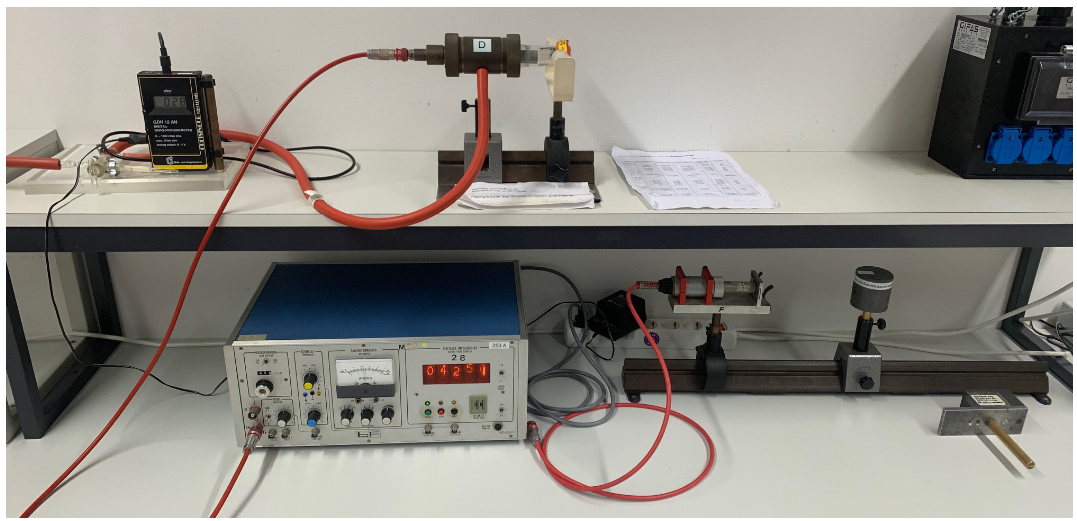
\includegraphics{graphics/aufbau.png}}
    \caption{Versuchsaufbau [Quelle: PAP2.2 Skript, S.75, Stand: 01.08.2024]}
    \label{fig:aufbau}
\end{figure}


\phantom{.}





%---------------VERSUCHSPROTOKOLL MIT MESSDATEN---------------
\newpage

\section{Versuchsprotokoll mit Messdaten}

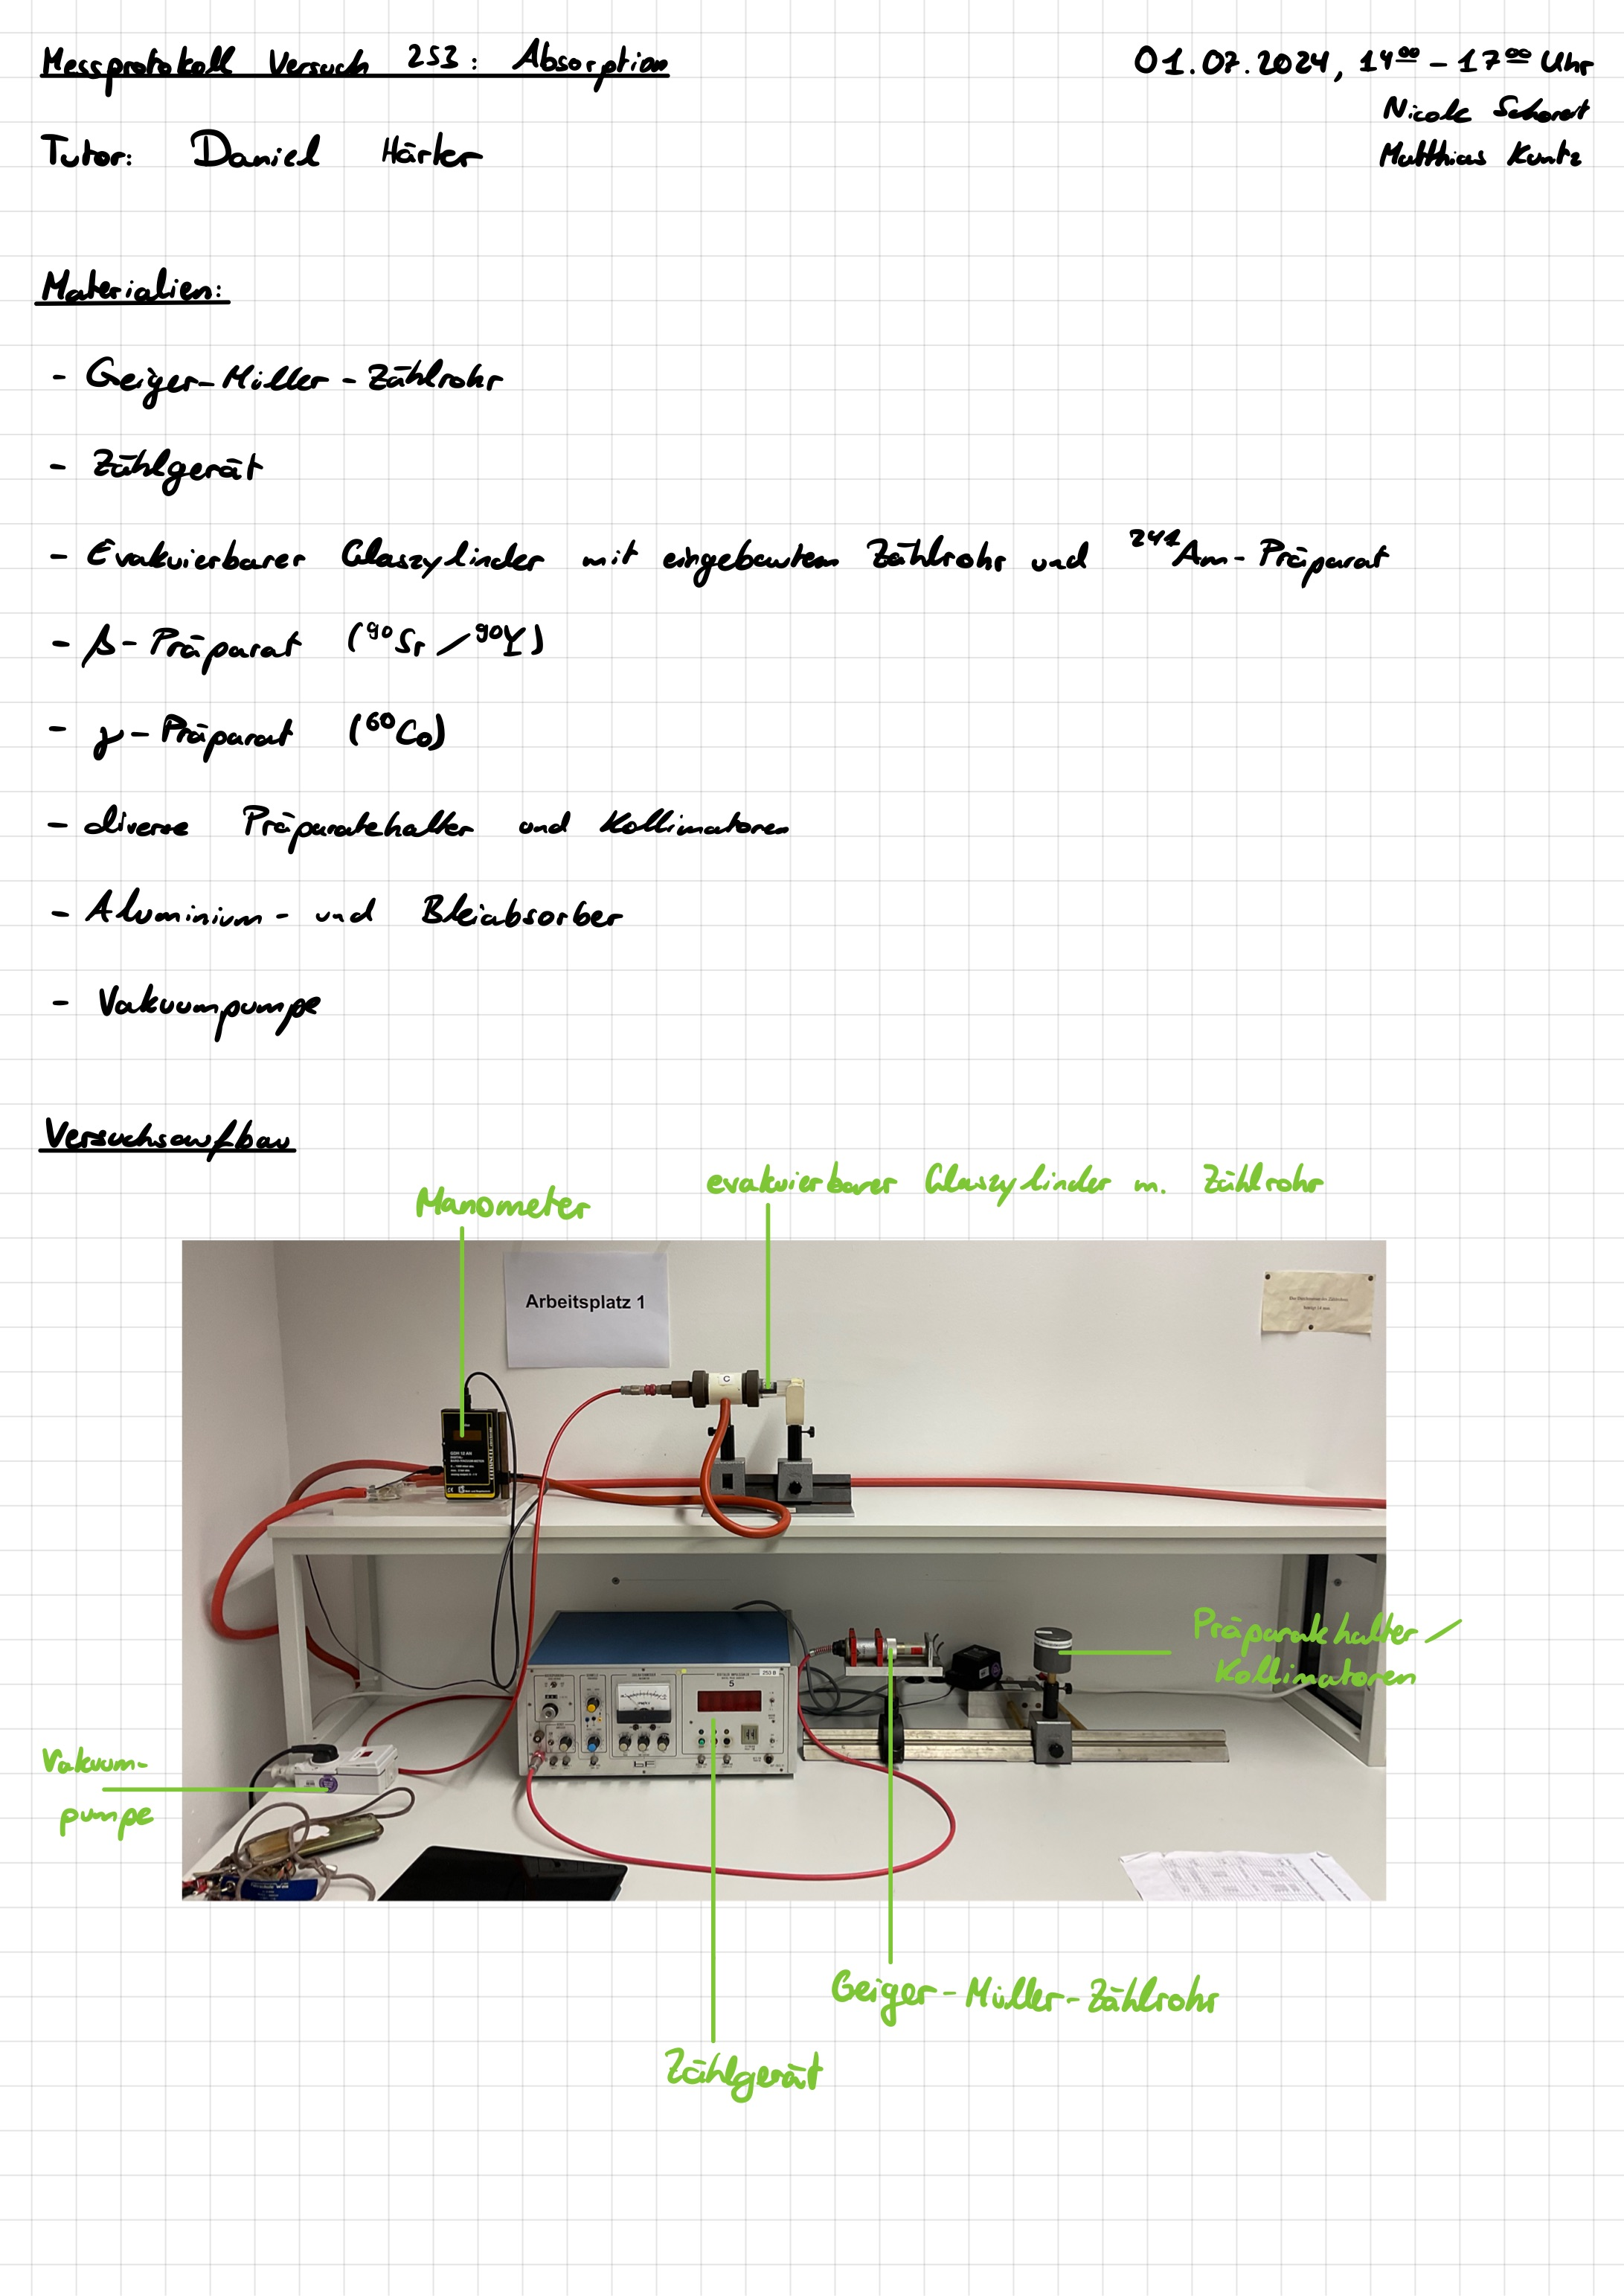
\includegraphics[width=\textwidth]{graphics/mess1.jpg}
\newpage
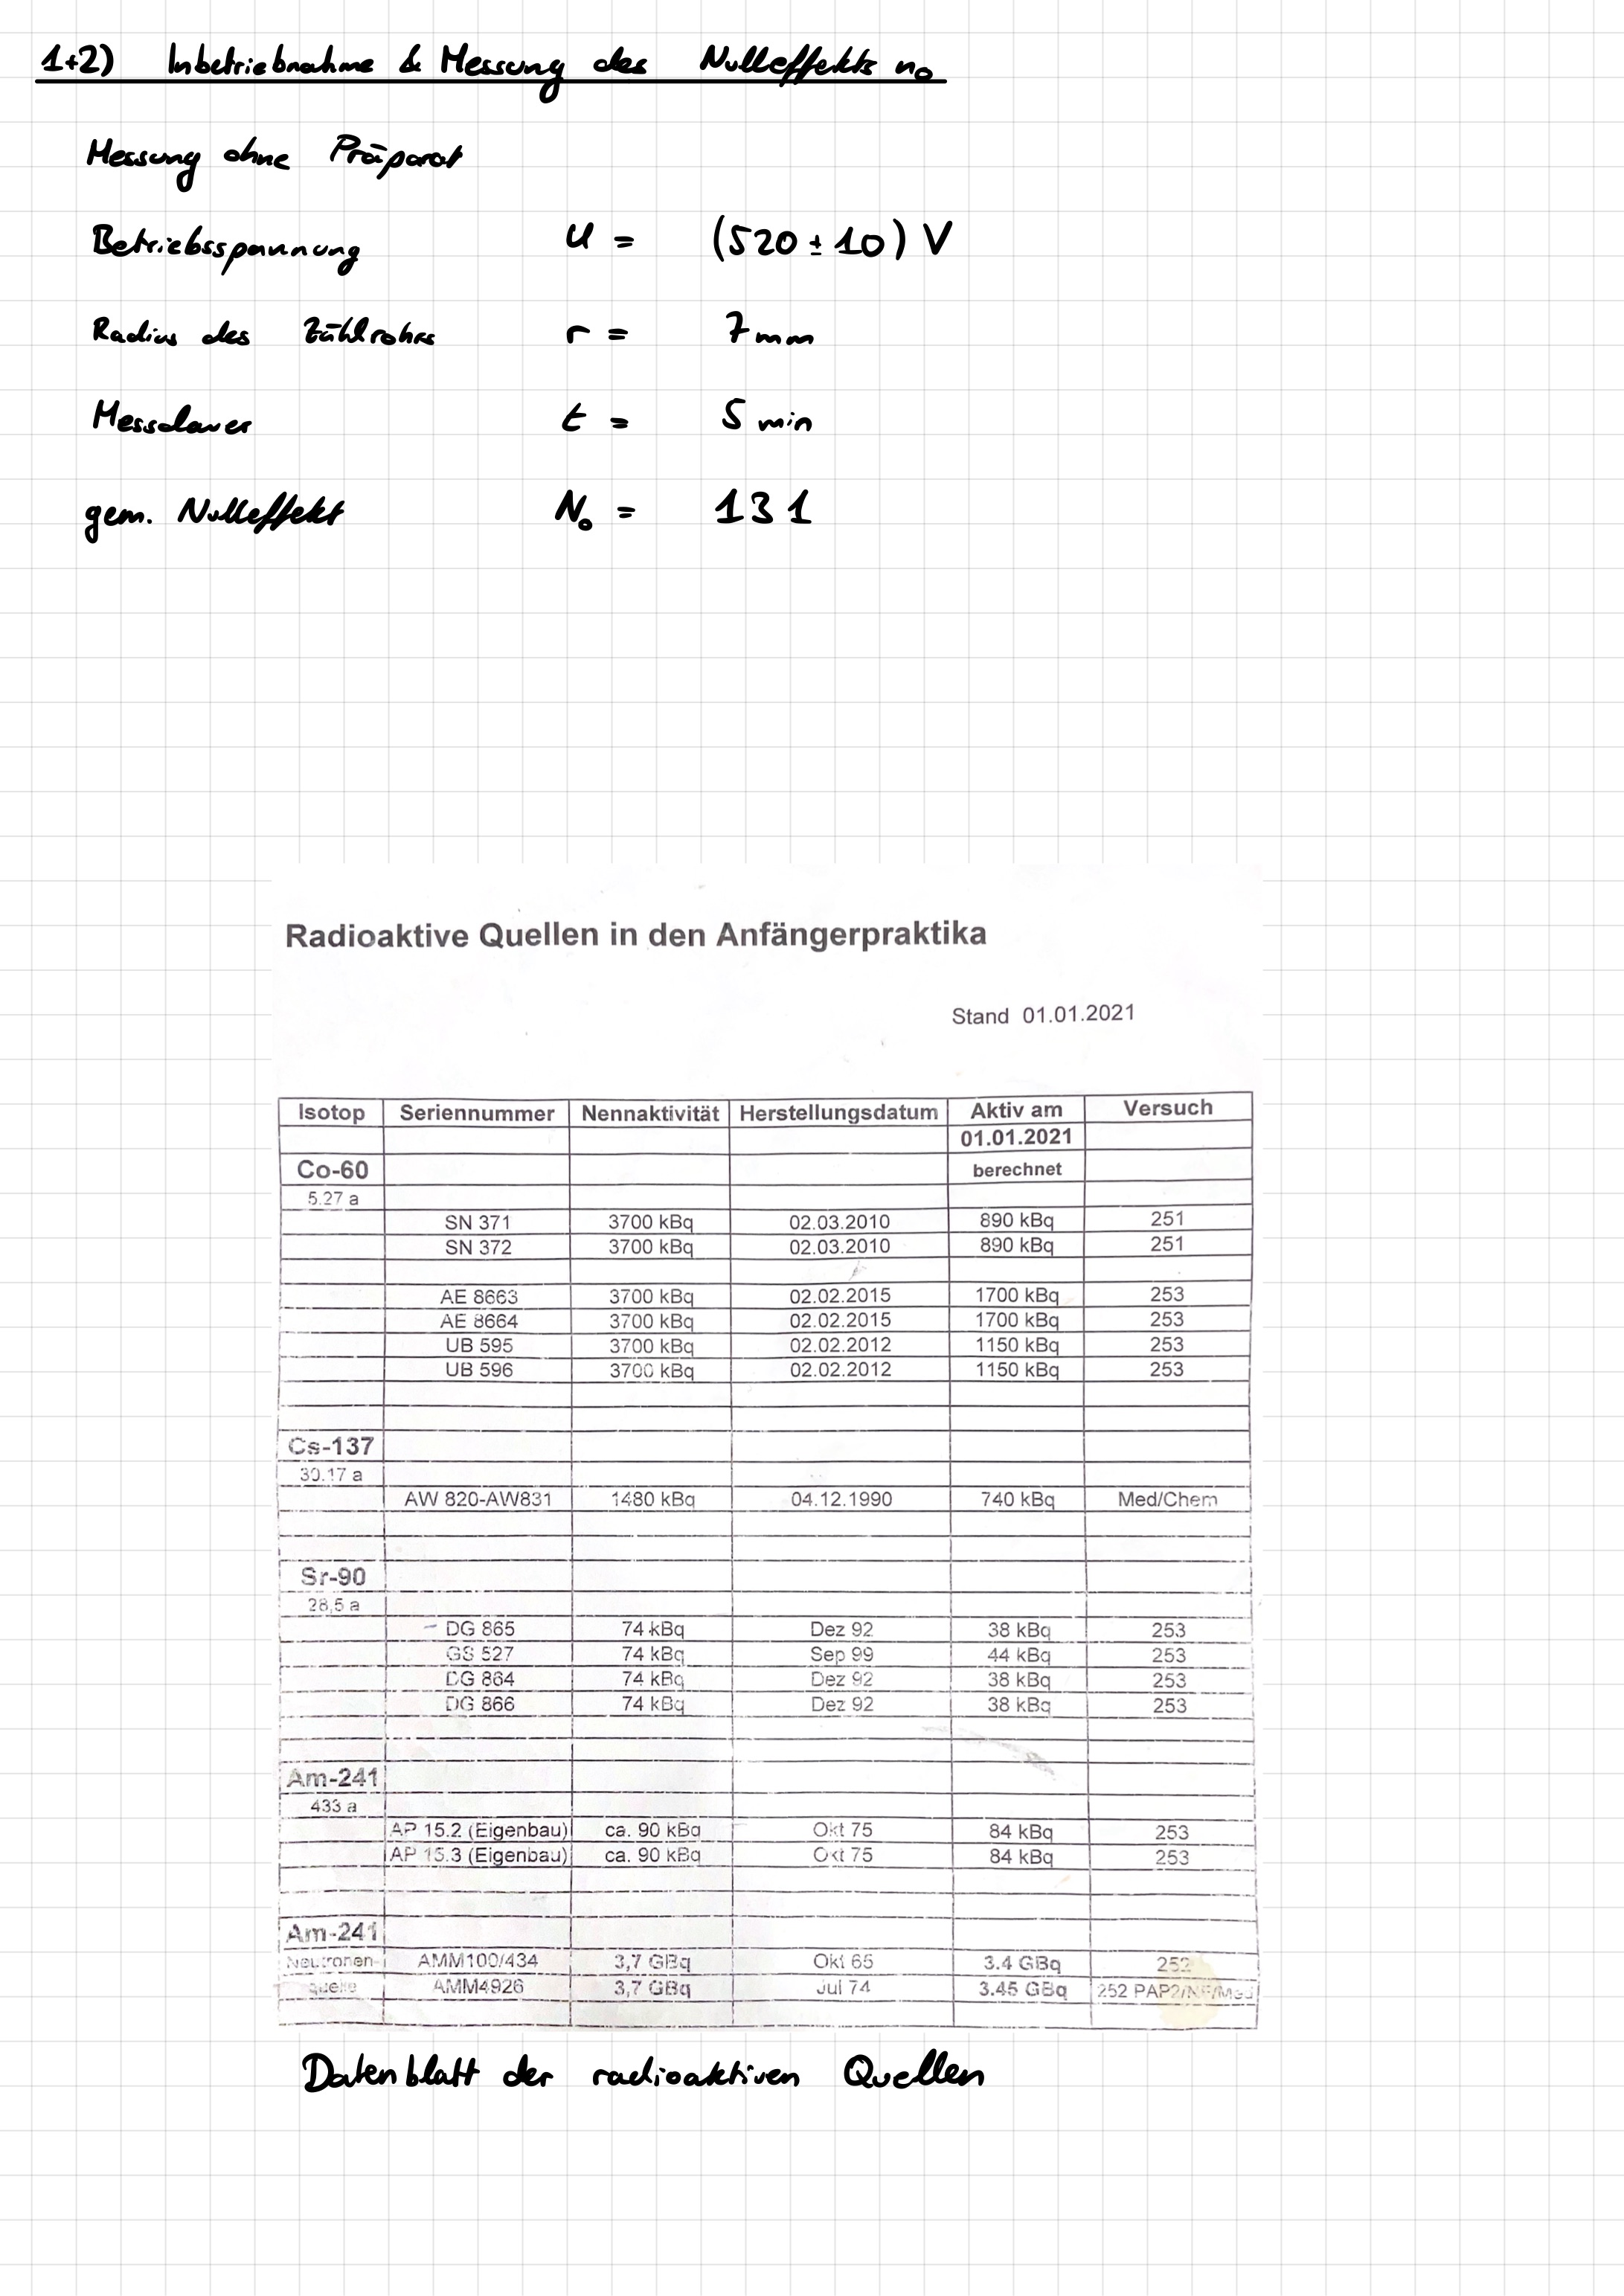
\includegraphics[width=\textwidth]{graphics/mess2.jpg}
\newpage
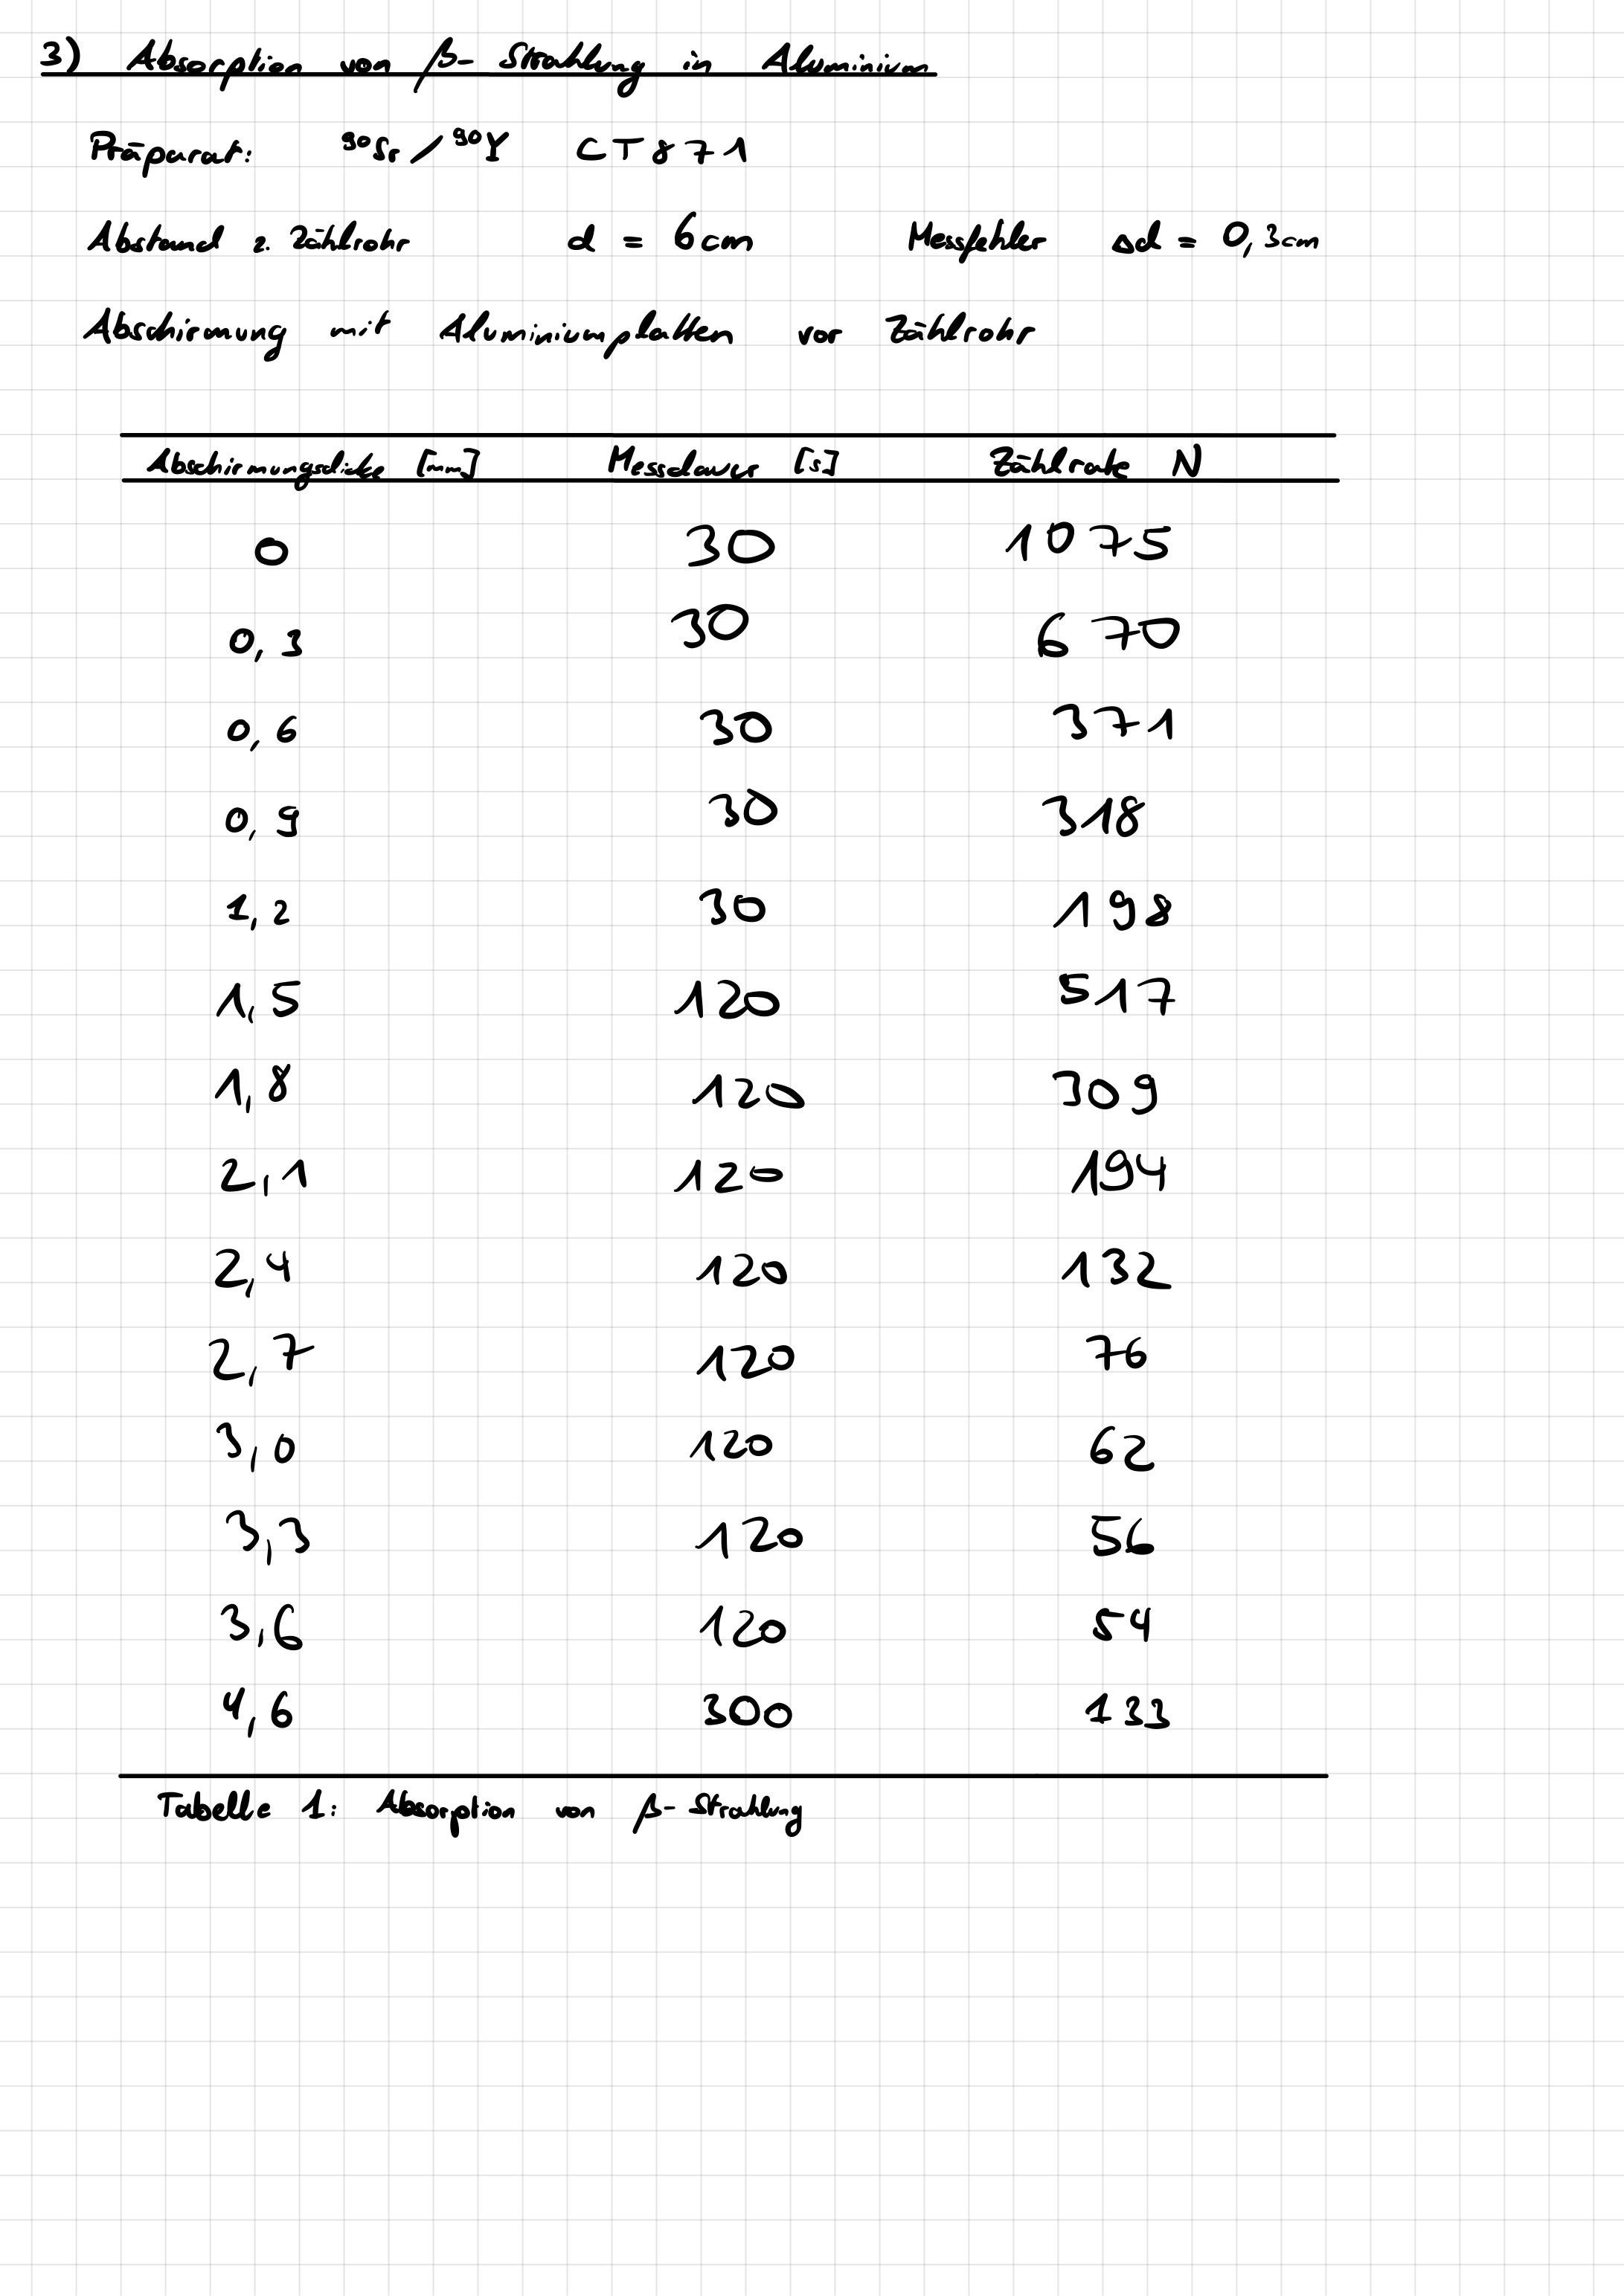
\includegraphics[width=\textwidth]{graphics/mess3.jpg}
\newpage
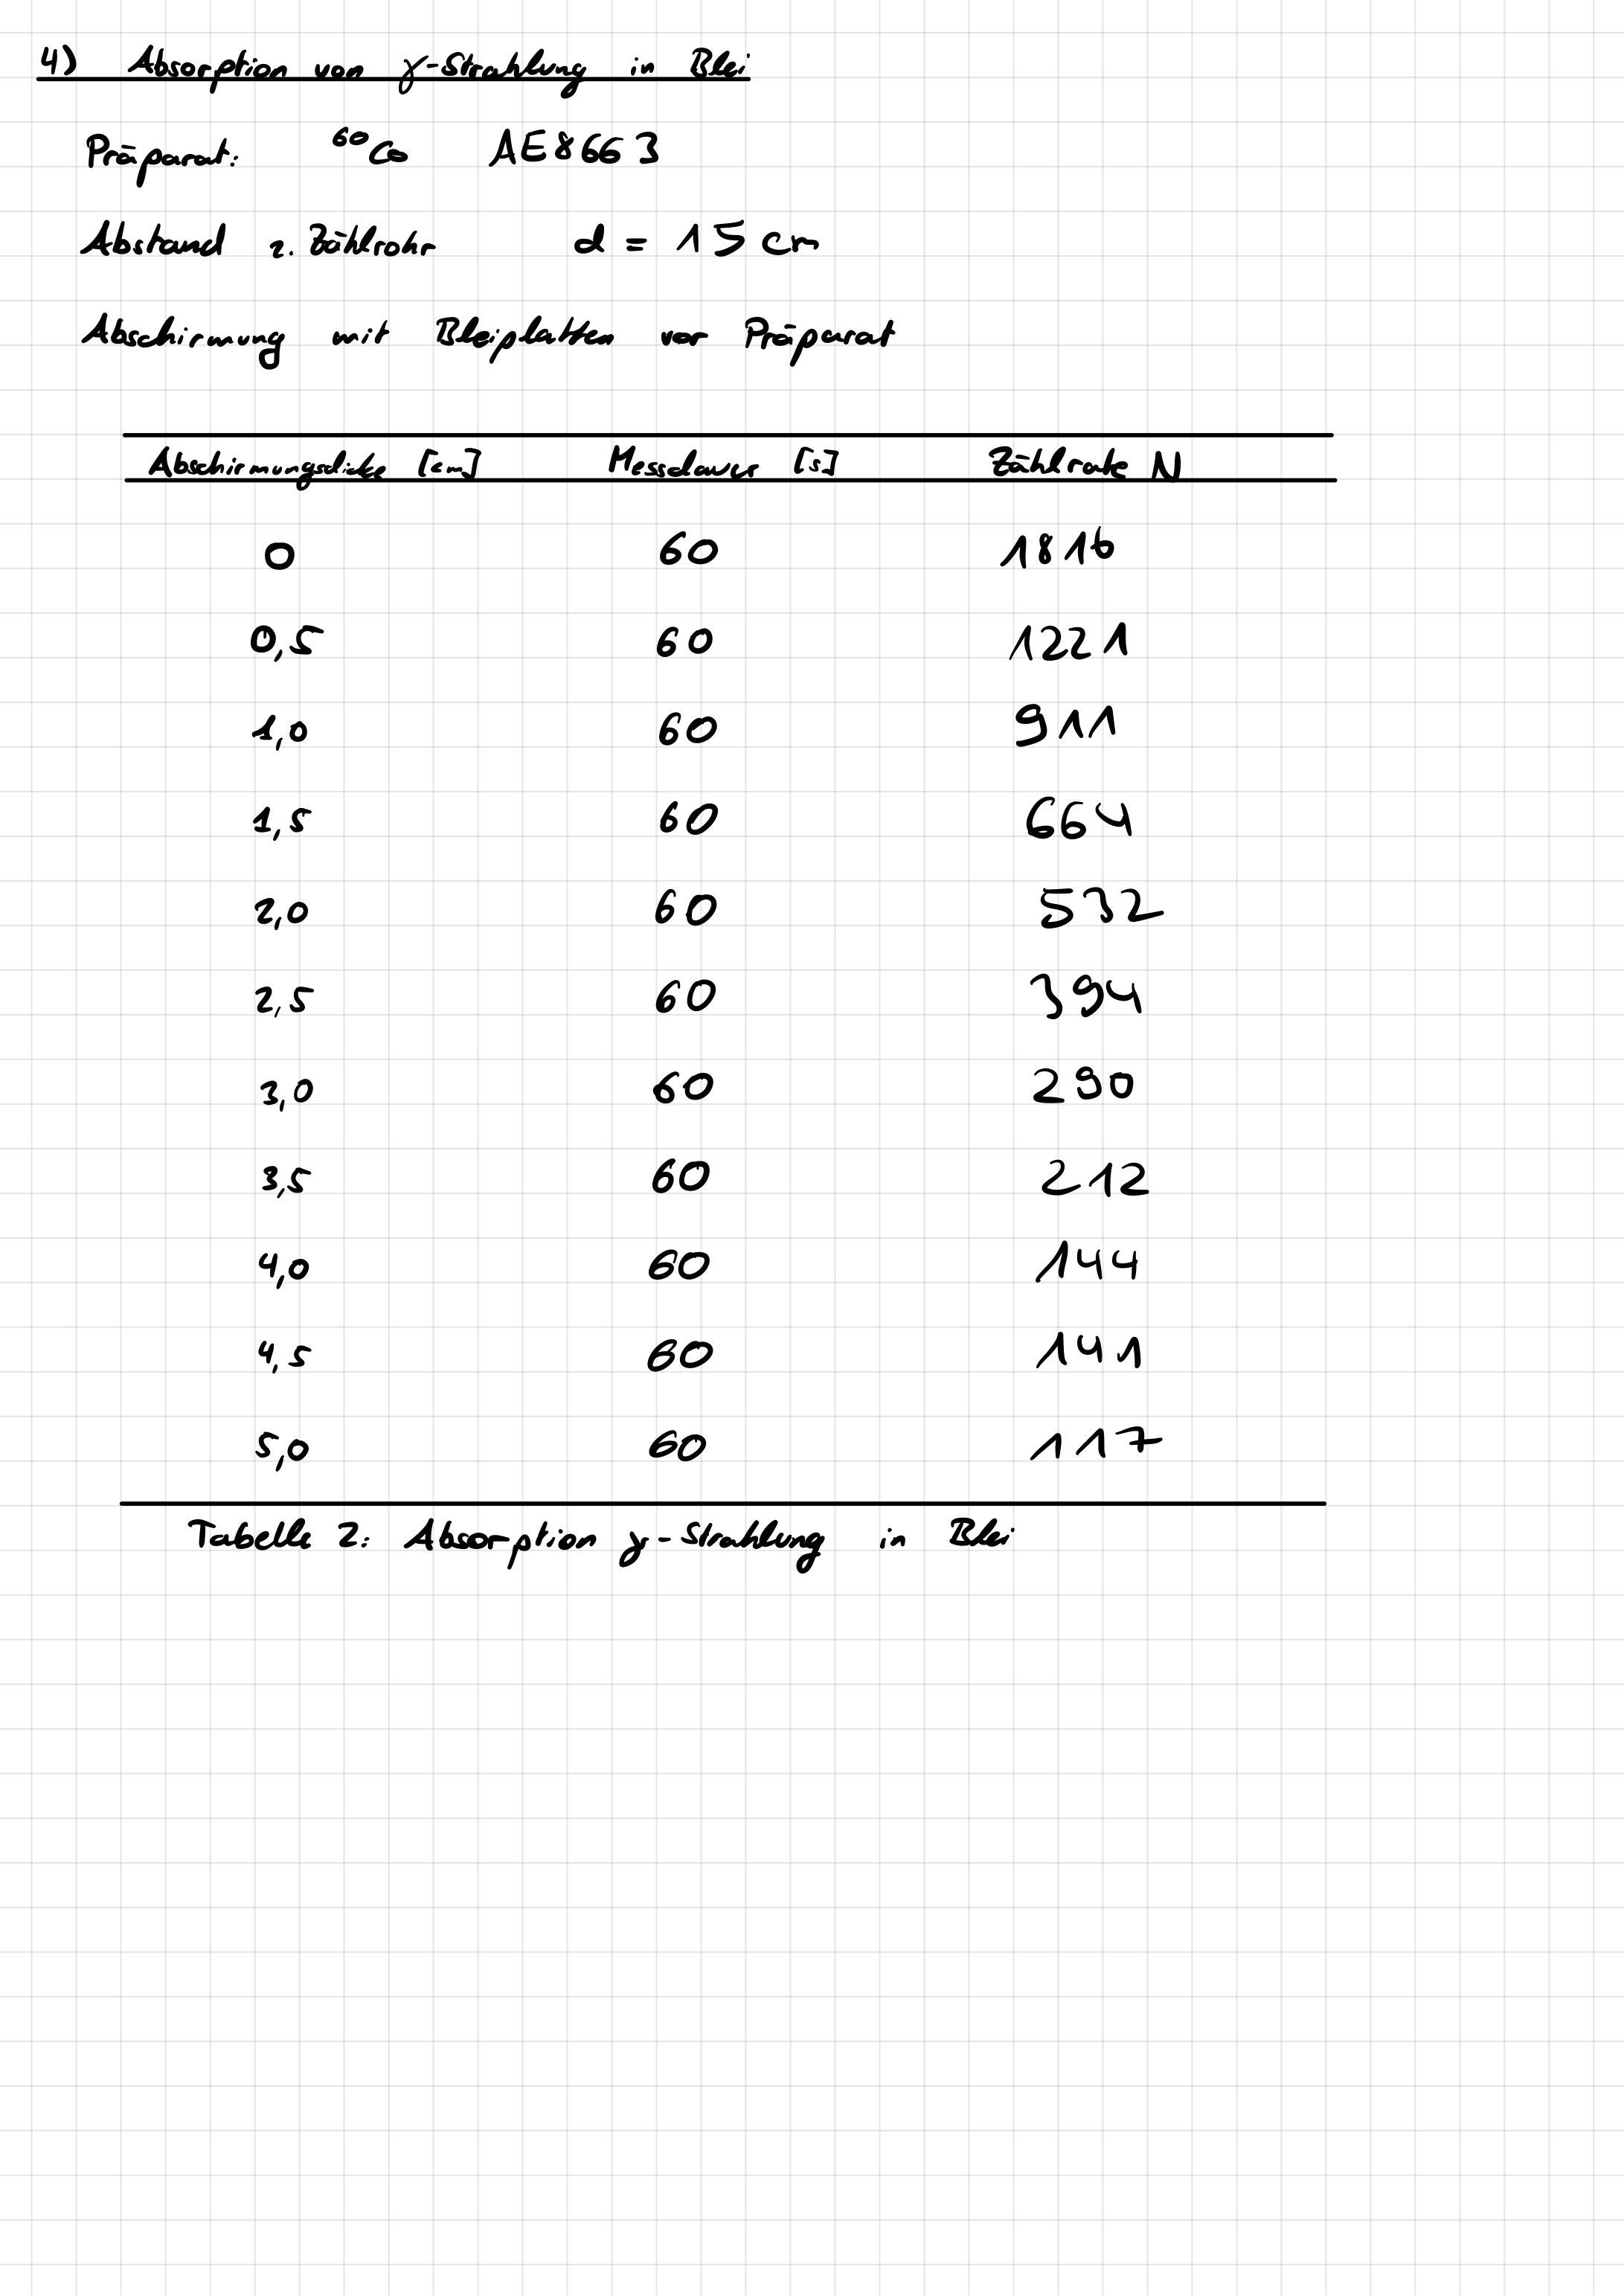
\includegraphics[width=\textwidth]{graphics/mess4.jpg}
\newpage
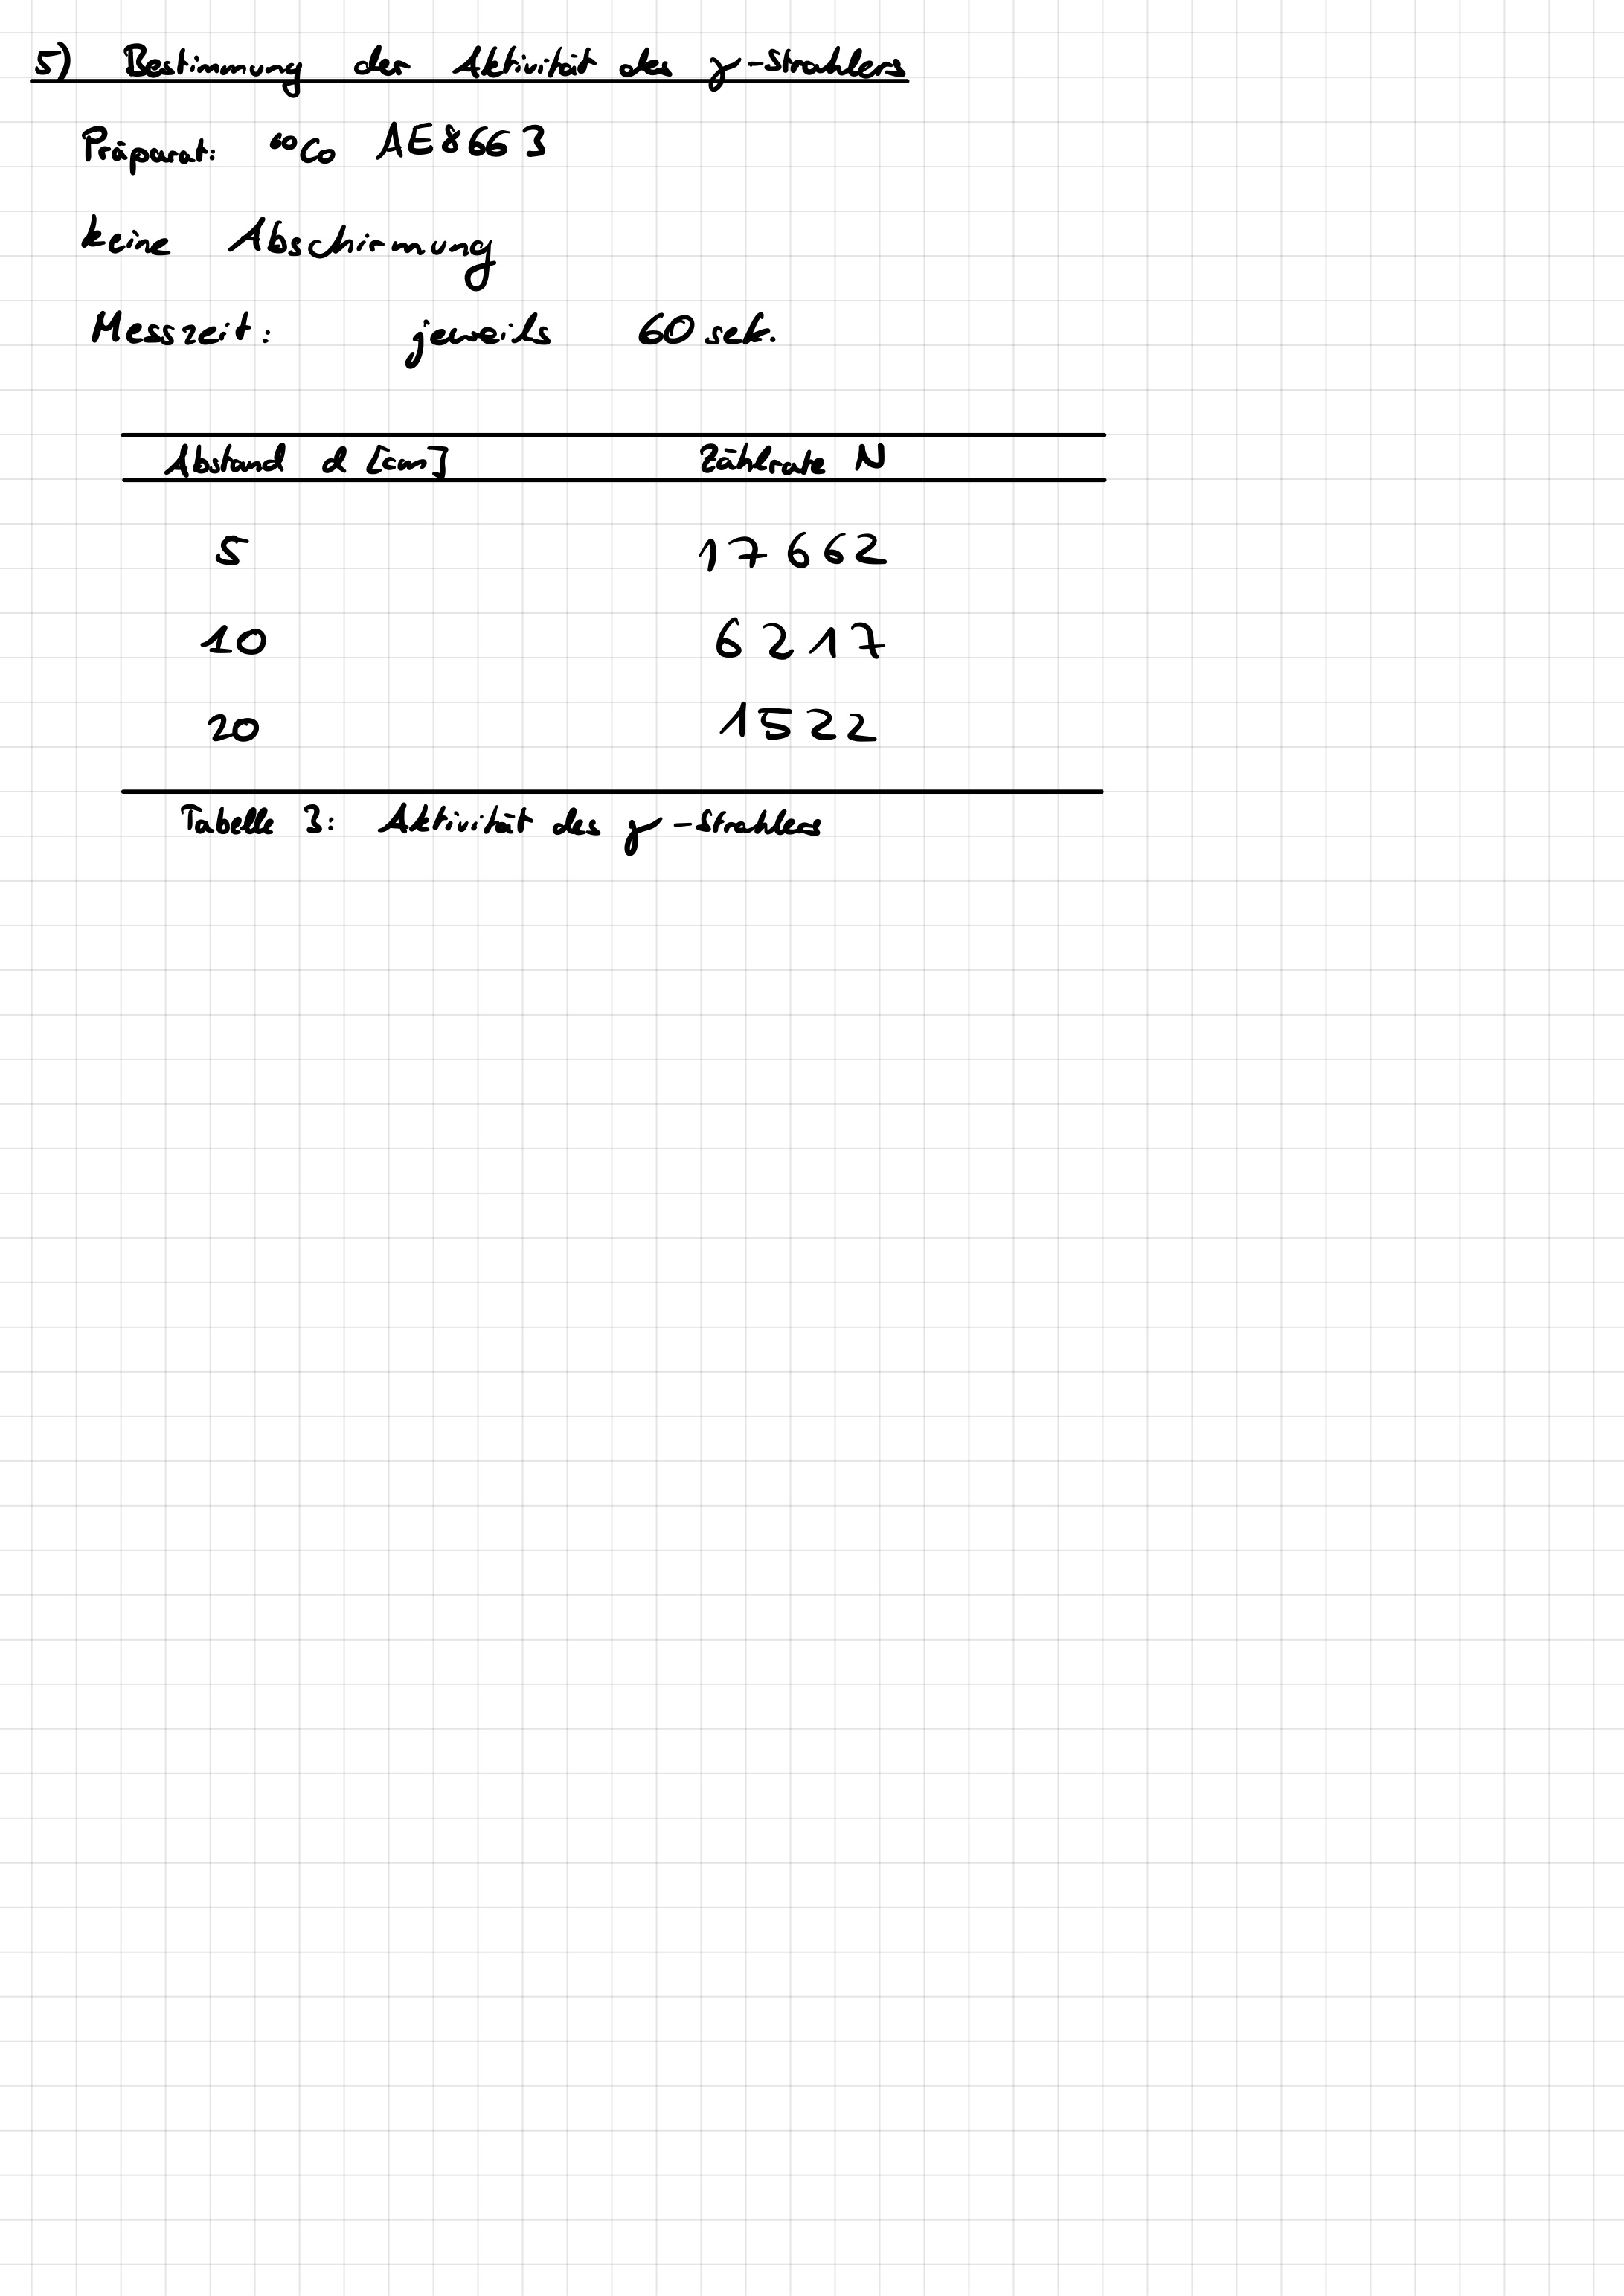
\includegraphics[width=\textwidth]{graphics/mess5.jpg}
\newpage
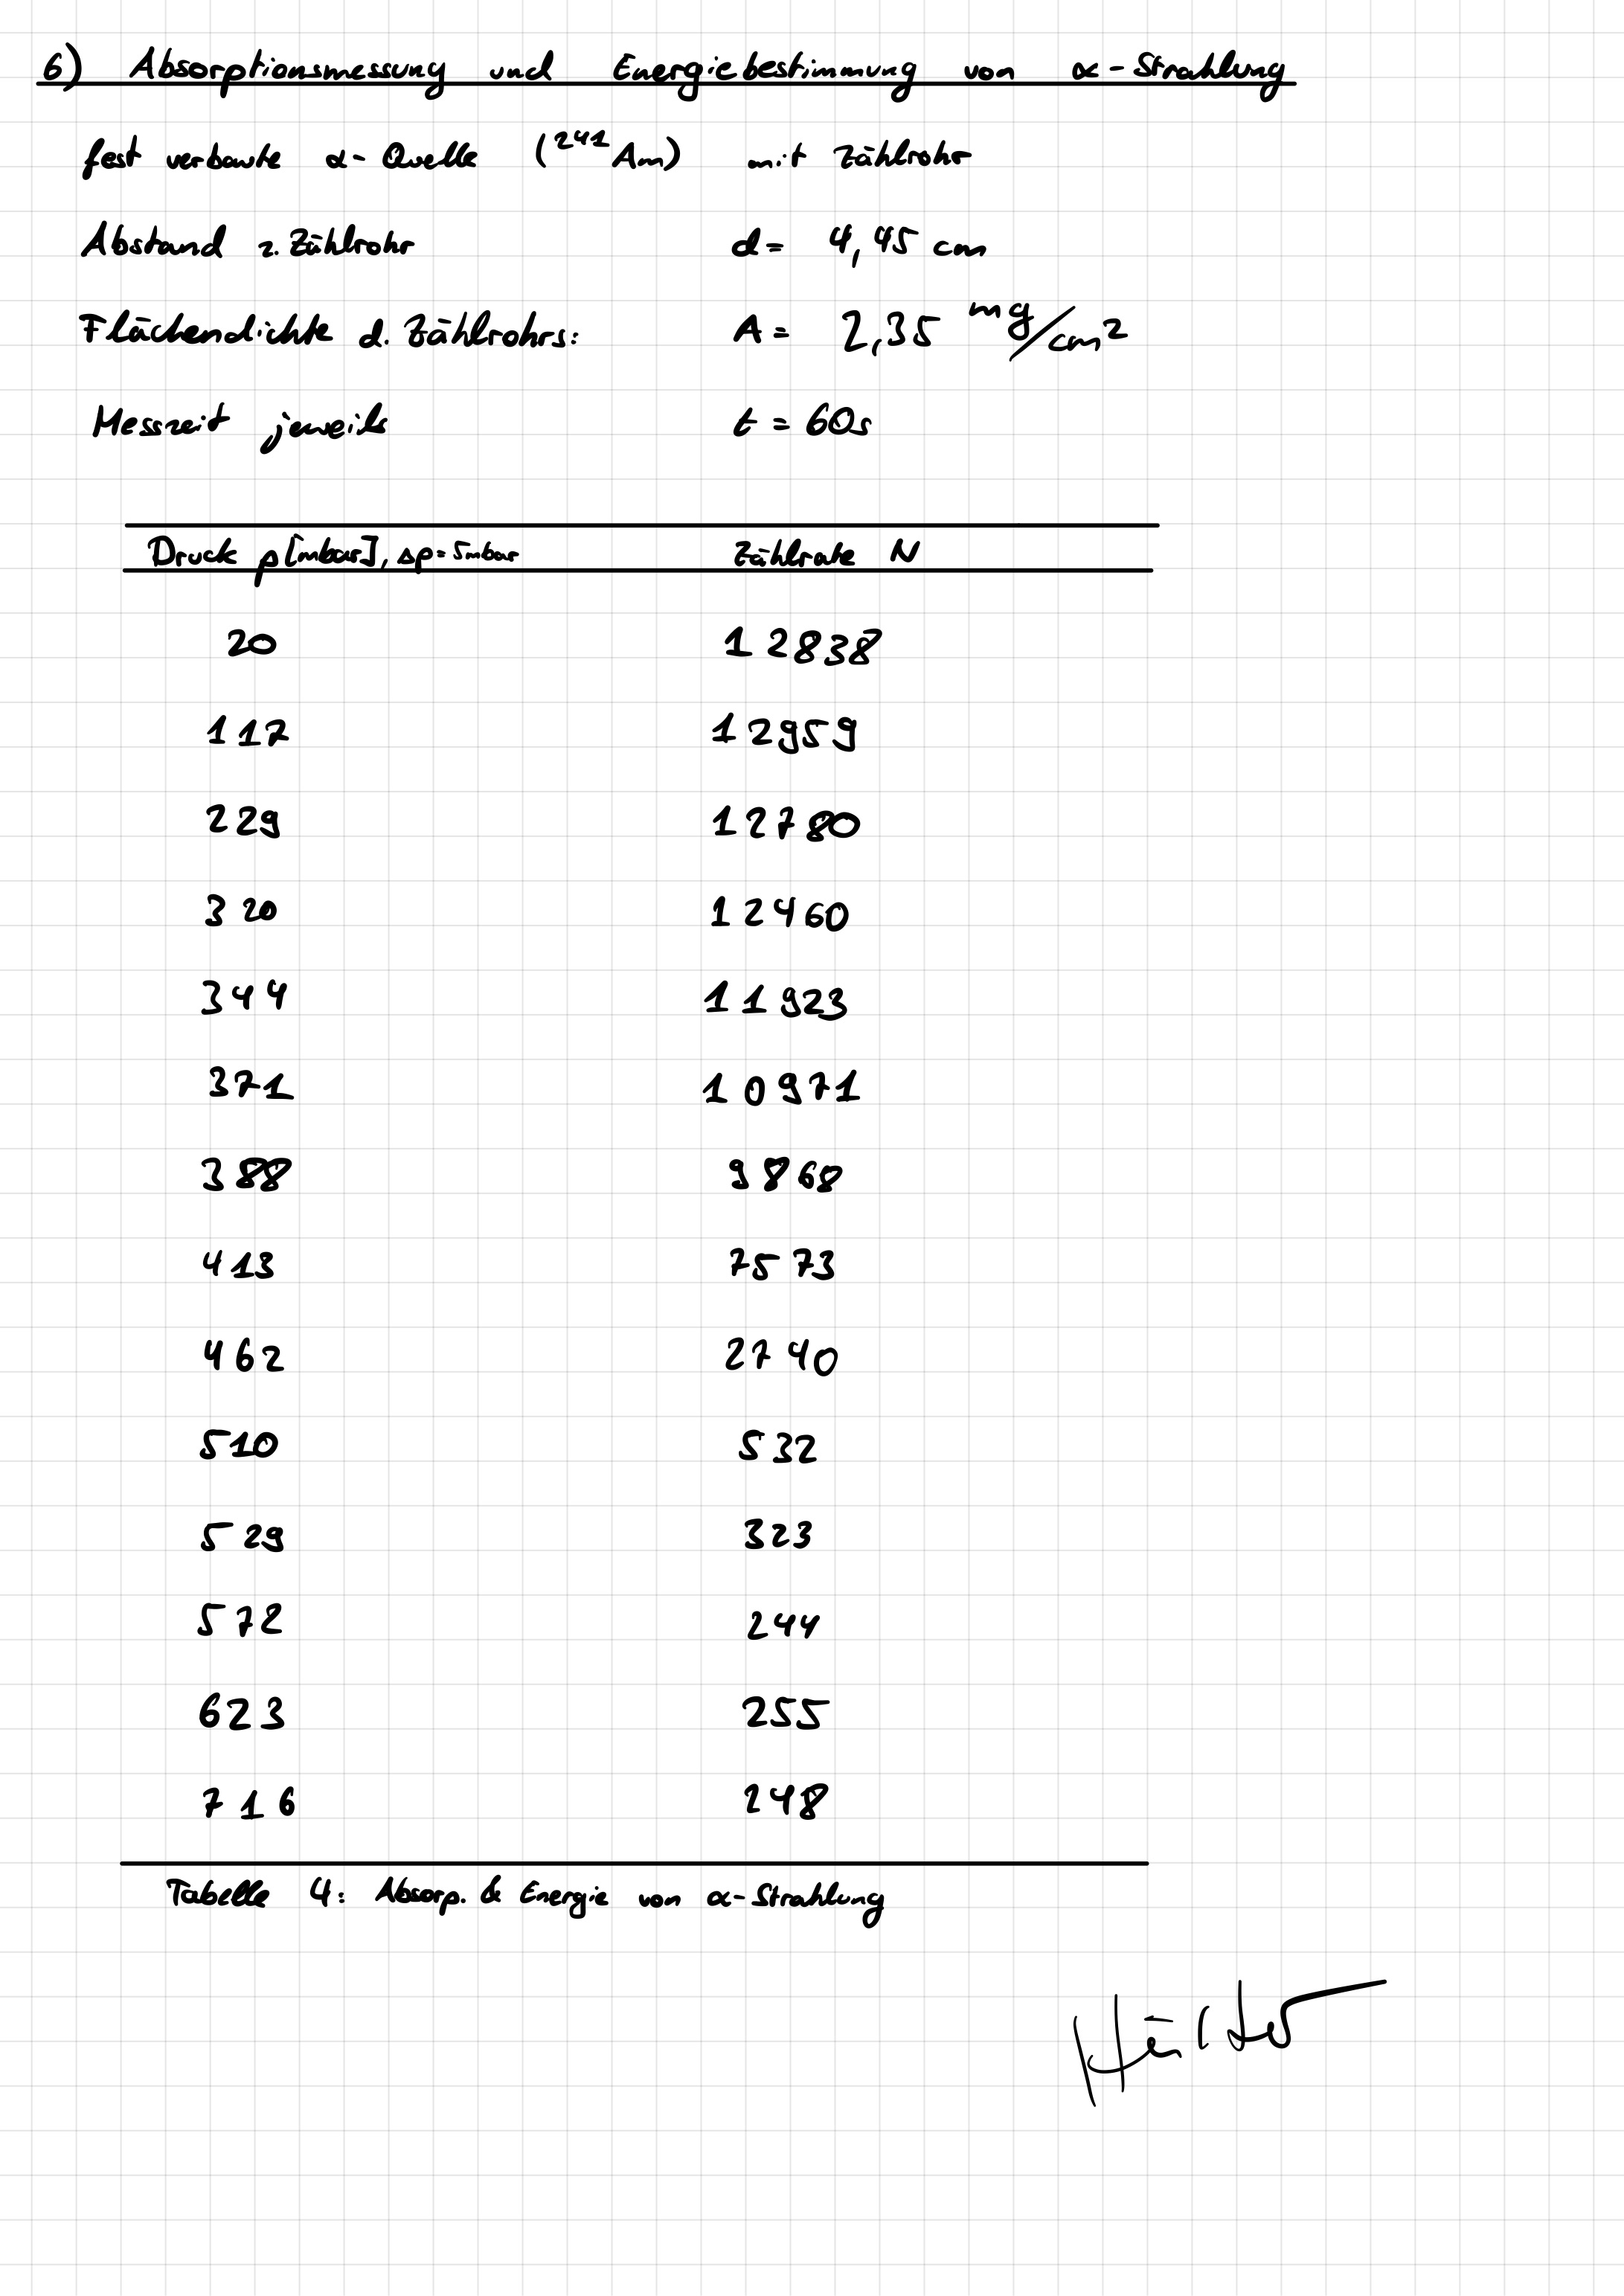
\includegraphics[width=\textwidth]{graphics/mess6.jpg}
\newpage

\addtocounter{table}{4}




\clearpage
\newpage
%-------------------------AUSWERTUNG-------------------------
\section{Auswertung}

In dieser Evaluation werden alle Fehler, sofern keine spezifische Angabe gemacht wird, mithilfe der Gauss'schen Fehlerfortpflanzung berechnet. Dies bedeutet, dass ein Wert $F$, der mit der Formel $f(a_1, ..., a_n)$ berechnet wird, den Fehler $\Delta F$ annimmt:

\begin{equation}
    \Delta F = \sqrt{\sum_n \left( \frac{\partial f}{\partial a_n} \cdot \Delta a_n \right)^2}.
\end{equation}

Des Weiteren erfolgen Signifikanztests von zwei Werten $a$ und $a'$ über die folgende Formel:

\begin{equation}
    \sigma = \frac{|a-a'|}{\sqrt{(\Delta a)^2 + (\Delta a')^2}}.
\end{equation}

Die Auswertung sowie Berechnung erfolgen über das dem Dokument angehängte Python-Programm. Hierbei erfolgen Fits von Funktionen mithilfe der 'curve\_fit'-Funktion des 'SciPy'-Packages und Plots werden mit 'matplotlib' erstellt.


\newpage

\subsection{Nulleffekt}

Zuerst berechnen wir aus den Messwerten des ersten Teils die Rate des Nulleffekts, da wir diese in den folgenden Versuchsteilen berücksichtigen werden. Aus den Messungen $N_0 = 131$ und $t=5$min berechnen wir:

\begin{equation}
    \begin{split}
        n_0 &= \frac{N_0}{t}, \ \ \ \ \ \Delta n_0 = \frac{\sqrt{N_0}}{t} \\ \\
        &\Rightarrow \bm{n_0 = (0,44 \pm 0,04)} \textbf{1/s}
    \end{split}
\end{equation}

\subsection{Absorption von $\beta$-Strahlung in Aluminium}

Wir berechnen die Raten $n$ aus den gemessenen Ereignissen $N$ aus Tabelle 1 des Messprotokolls und ziehen den bestimmten Nullwert $n_0^\beta$ ab. Die so resultierenden Zählraten plotten wir als Funktion der Absorberdicke in halblogarithmischem Maßstab und können nun an den Verlauf eine Exponentialfunktion fitten, die aufgrund des halblogarithmischen Maßstabs bei der Maximalreichweite im Medium nahezu senkrecht verläuft. Indem wir zusätzlich eine obere und untere Fehlerkurve anlegen am oberen und unteren $1\sigma$-Bereich der Fitparameter können wir den Fehler abschätzen. Das Diagramm mit allen Fits ist in Abbildung \ref{fig:A3-Reichweite} dargestellt.

\begin{figure}[!h]
    \centering
    \resizebox{0.9\textwidth}{!}{
    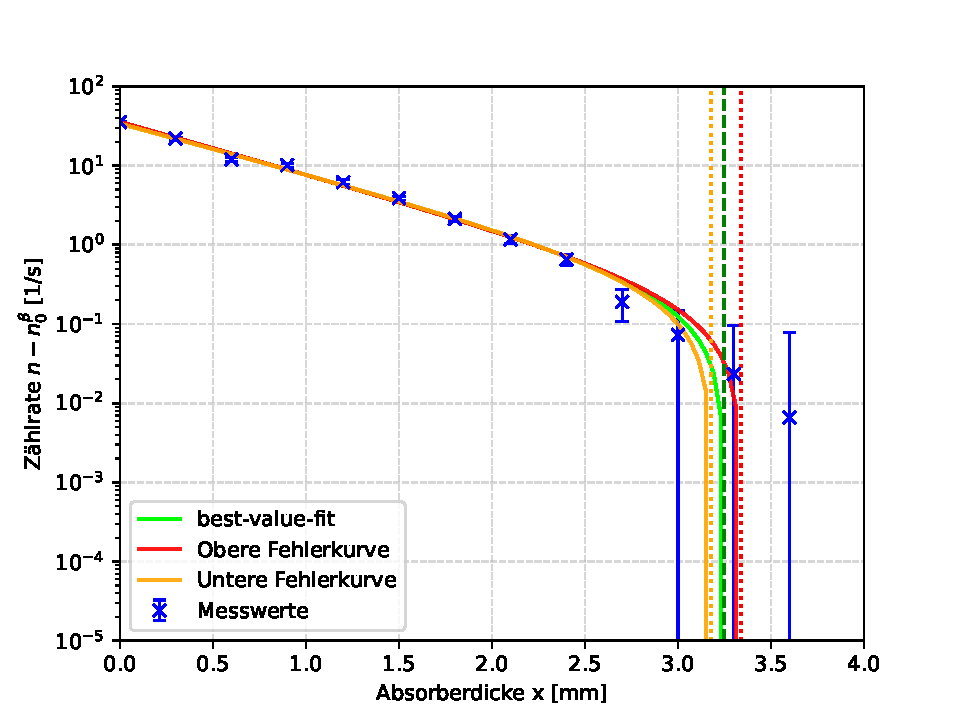
\includegraphics{plots/Maximalreichweite-beta.pdf}}
    \caption{Bestimmung Maximalreichweite von $\beta$-Strahlung in Aluminium}
    \label{fig:A3-Reichweite}
\end{figure}

Indem wir die Schnittpunkte der drei Exponentialfunktionen mit einer sehr kleinen Konstanten (10$^{-5}$) berechnen, erhalten wir den folgenden Wert für die Maximalreichweite:  

\begin{equation}
    d_{max} = 3,25 ^{+0,09} _{-0,07} \ \text{mm}
\end{equation}

Mit diesem Wert können wir die Flächendichte $R^\beta$ bestimmen. Dazu benötigen wir die Flächendichte der Präparatskapsel von $R^\beta _{ES} = 0,130$g/cm$^2$ und die Dichte von Aluminum $\rho_{Al} = 2.71$g/cm$^3$. Wir erhalten:

\begin{equation}
    \begin{split}
        R^\beta &= \rho_{Al} \cdot d_{max} + R^\beta _{ES} \\
        \Rightarrow \Delta R^\beta &= \rho_{Al} \cdot \Delta d_{max} \\ \\
        &\Rightarrow R^\beta = 1,010 ^{+0,024} _{-0,018} \ \text{g/cm}^3
    \end{split}
\end{equation}

Wir nutzen diesen Wert, um aus Diagramm \ref{fig:Anhang-Reichweite} im Anhang die Maximalenergie der $\beta$-Teilchen zu ermitteln. Wir lesen dabei den folgenden Wert ab:

\begin{equation}
    \bm{E_{\beta,max} = (2,2 \pm 0,1)} \textbf{MeV}
\end{equation}

Verglichen mit dem Literaturwert 2,274 MeV ergibt sich eine insignifikante Abweichung von $0,74\sigma$, was unser Ergebnis und die verwendeten Messwerte sowie Methoden bestätigt. 

\clearpage
\newpage

\subsection{Absorption von $\gamma$-Strahlung in Blei}

Wir berechnen aus den Messwerten in Tabelle 2 die Raten und ziehen den anfangs berechneten Nulleffekt $n_0$ ab. Wir stellen die resultierenden Raten erneut in einem halblogarithmischem Diagramm dar und fitten eine dem Beere-Lambert-Gesetz (\ref{eq:Lambert-Beere}) entsprechende Exponentialfunktion, zu sehen in Abbildung ref{fig:A4-AbsorptionGamma}. Dabei erhalten wir den Fitparameter für den Schwächungskoeffizient $\mu = (0,630 \pm 0,011)$1/cm, welchen wir mit der Dichte von Blei $\rho_{Pb} = 11.342$g/cm$^3$ in den Massenschwächungskoeffizient $\mu / \rho$ umrechnen:

\begin{equation}
    \frac{\mu}{\rho} = (0,0555 \pm 0,0010) \text{cm}^2 \text{/g}
\end{equation}

Mit diesem Wert lesen wir aus Diagramm \ref{fig:Anhang-PhotonCrossSection} im Anhang die Energie der emittierten $\gamma$-Quanten und erhalten:

\begin{equation}
    \bm{E_\gamma = (1.4 \pm 0.2)} \textbf{MeV}
\end{equation}

Wir vergleichen erneut mit dem Literaturwert, der diesmal 1,333 MeV beträgt, und erhalten erneut eine insignifikante Abweichung von $0,33\sigma$.



\begin{figure}[!b]
    \centering
    \resizebox{0.9\textwidth}{!}{
    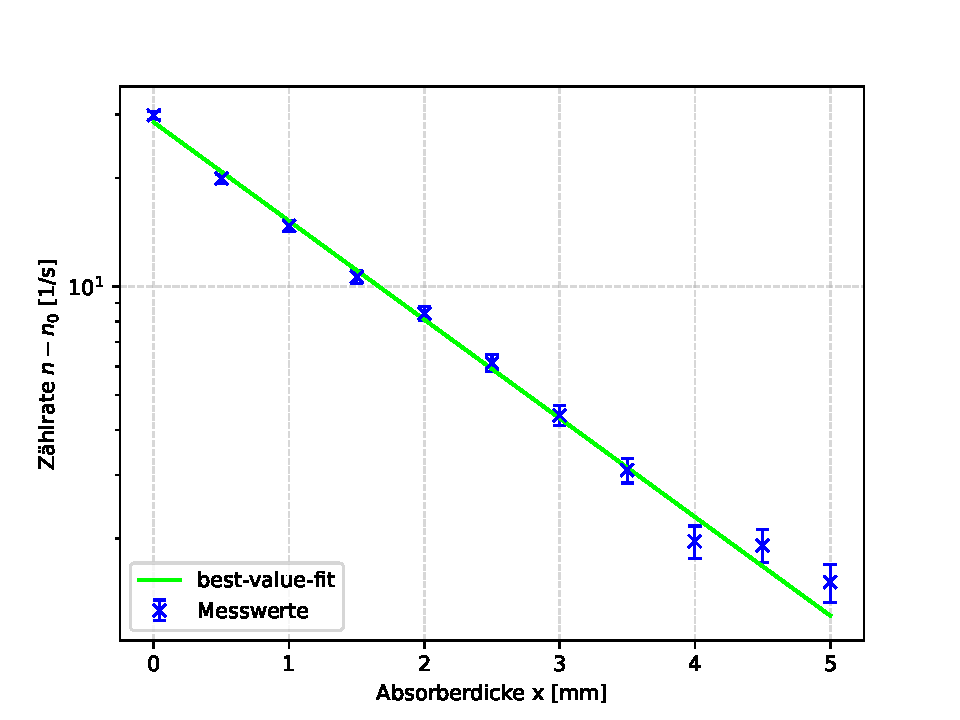
\includegraphics{plots/Absorption-gamma.pdf}}
    \caption{Absorption von $\gamma$-Strahlung in Blei}
    \label{fig:A4-AbsorptionGamma}
\end{figure}

\clearpage
\newpage

\subsection{Aktivität des $\gamma$-Strahlers}

Wir beginnen, indem wir die genäherten Aktivitäten bei den drei Distanzen berechnen. Dazu bestimmen wir die Raten aus den Messwerten in Tabelle 3, ziehen von denen den Nulleffekt $n_0$ ab und halbieren die resultierenden Werte, da pro Zerfall zwei Photonen entstehen. Wir verwenden Gleichung \ref{eq:Aktivität-ohneKorr}, um die unkorrigierten Aktivitäten zu bestimmen, wobei sich der Fehler folgendermaßen berechnet:

\begin{equation}
    \Delta A = A \sqrt{\left(\frac{\Delta n}{n}\right)^2 + \left(\frac{\Delta d}{d}\right)^2}
\end{equation}

Zum Vergleich bestimmen wir die Nennaktivität zum Tag des Versuchs mit dem Datenblatt des Messprotokolls. Bei einer Halbwertszeit von 5,27 Jahren und einer Zeit von exakt 3,5 Jahren seit der letzten protokollierten Aktivität von 1700 kBq vom 01.01.2021 erhalten wir den folgenden Wert für die theoretische Aktivität zum Versuchstag:

\begin{equation}
    A_{theo} = 1700 \text{kBq} \cdot e^{- \ln{(2)} \frac{t}{T_{1/2}}} = 1072,812 \text{kBq}
\end{equation}

Die Aktivitäten mit dem Literaturwert und Signifikanztests sind in Tabelle \ref{tab:A5-ohneKorr} eingetragen.

\begin{table}[!h]
    \centering
    %\resizebox{\textwidth}{!}{
    \begin{tabular}{cccc}
        \hline
        $\bm{d}$ [cm] & $\bm{A}$ [MBq] & $\bm{A_{theo}}$ [MBq] & $\bm{\sigma}$  \\ \hline
         5  & 0,75 $\pm$ 0,05 & 1,072812 & 7,12 \\
         10 & 1,05 $\pm$ 0,03 & 1,072812 & 0,58 \\
         20 & 1,02 $\pm$ 0,03 & 1,072812 & 1,80 \\ \hline
    \end{tabular}%}
    \caption{Aktivität ohne Korrektur}
    \label{tab:A5-ohneKorr}
\end{table}

Wir berechnen nun noch die korrigierten Aktivitäten gemäß Gleichungen \ref{eq:Längenkorrektur} und \ref{eq:Absorptionskorrektur}. Die Länge des Zählrohrs ist gegeben als 4 cm und für die Absorptionskorrektur verwenden wir die Dicke $x = 1,4$mm sowie Dichte $\rho = 7,9$g/cm$^3$ der Präparatskapsel und bestimmen den Schwächungskoeffizient $\mu'$ gemäß

\begin{equation}
    \mu' = \frac{\mu}{\rho_{Pb}} \rho_{Absorber} = (43,9 \pm 0,8) \text{1/m},
\end{equation}

wobei wir das Verhältnis $\mu / \rho$ aus Teil 4 verwenden. 

Die Raumwinkelkorrektur beläuft sich also auf:

\begin{equation}
    \begin{split}
        A_{corr,1} &= n \cdot k_{corr} = n \cdot \frac{4 (d+l/2)^2}{\varepsilon r^2}, \\
        \Rightarrow \Delta k_{corr} &= \Delta d \cdot 2 \frac{4 (d+l/2)}{\varepsilon r^2}, \\
        \Delta A_{corr,1} &= A_{corr,1} \sqrt{(n \cdot \Delta k_{corr})^2 + (k_{corr} \cdot \Delta n)^2}.
    \end{split}
\end{equation}

Und die Absorptionskorrektur ergibt:

\begin{equation}
    \begin{split}
        A_{corr,2} &= A_{corr,1} \cdot e^{\mu' \cdot x}, \\
        \Rightarrow \Delta A_{corr,2} &= \sqrt{\left(\Delta A_{corr,1} \cdot e^{\mu' \cdot x}\right)^2 + \left(x A_{corr,1} \cdot e^{\mu' \cdot x} \cdot \Delta \mu' \right)}.
    \end{split}
\end{equation}


Somit erhalten wir nach Anwenden der Korrekturen die in Tabelle \ref{tab:A5-mitKorr} dargestellten Ergebnisse und Signifikanztests.

\begin{table}[!h]
    \centering
    %\resizebox{\textwidth}{!}{
    \begin{tabular}{cccc}
        \hline
        $\bm{d}$ [cm] & $\bm{A}$ [MBq] & $\bm{A_{theo}}$ [MBq] & $\bm{\sigma}$  \\ \hline
         5  & 1,48 $\pm$ 0,13 & 1,072812 & 3,19 \\
         10 & 1,53 $\pm$ 0,08 & 1,072812 & 5,75 \\
         20 & 1,24 $\pm$ 0,05 & 1,072812 & 3,55 \\ \hline
    \end{tabular}%}
    \caption{Aktivität mit Korrektur}
    \label{tab:A5-mitKorr}
\end{table}

Es ist zu erkennen, das der erste Wert eine kleine Abweichung zum Literaturwert hat, dafür die letzten beiden aber deutlich weiter entfernt liegen. Allgemein weisen alle Werte signifikante Abweichungen zum berechneten Referenzwert auf. Woran das liegen könnte, lässt sich nur schwer sagen. Es lässt sich aber feststellen, dass die Aktivitäten an sich näher beieinander liegen als ohne Korrektur, was auch an sich zu erwarten ist. Die Raumwinkelkorrektur wird für größere Abstände nämlich immer geringer, da $(d+l/2)$ für große Abstände einfach gegen $d$ geht und somit der Korrekturfaktor gegen 1 geht und die verschiedenen Abstände ausgleicht. Insgesamt weisen die Korrekturen aber eher unzufriedenstellende Ergebnisse auf, da sie diese bis auf einen Wert nicht verbessert haben, was auf einen gröberen Mess- oder Methodikfehler hinweist

\clearpage
\newpage

\subsection{Absorption von $\alpha$-Strahlung in Luft}

Aus den Messwerten in Tabelle 4 bestimmen wir die Raten $n$ und tragen diese als Funktion des Drucks in ein Diagramm auf. Wir möchten nun den Druck bestimmen, an dem die Zählrate auf die Hälfte des Anfangswertes im Vergleich zum Endwert gesunken ist. 
Wir berücksichtigen hierbei den Endwert, um die Hintergrundeffekte nicht mitzubeachten. Dazu fitten wir eine Funktion an, die dem ungefähren Verlauf der Messwerte entspricht:

\begin{equation}
    y = \frac{\alpha}{10 + e^{-\beta (x - x_0)}} + bkg.
\end{equation}

Wir erhalten das in Abbildung \ref{fig:A6-Alpha} dargestellte Diagramm, aus welchem wir manuell den Schnittpunk mit der halben Zählrate von 105 1/s bestimmen und somit den folgenden Druck erhalten:

\begin{equation}
    p = (423 \pm 3) \text{mbar}
\end{equation}

\begin{figure}[!b]
    \centering
    \resizebox{0.9\textwidth}{!}{
    \includegraphics{plots/Aktivität-alpha.pdf}}
    \caption{Absorption von $\alpha$-Strahlung in Luft}
    \label{fig:A6-Alpha}
\end{figure}

Damit berechnen wir die Reichweite $s_1$ der $\alpha$-Strahlung bei dem gegebenen Druck, wofür wir den Normaldruck $p_0 = 1013$mbar und den Abstand vom Präparat zum Zählrohr $s_0 = (3,95 \pm 0,05)$cm benötigen:

\begin{equation}
    \begin{split}
        s_1 &= \frac{p}{p_0} s_0 \\
        \Rightarrow \Delta s_1 &= s_1 \sqrt{\left(\frac{\Delta s_0}{s_0}\right)^2 + \left(\frac{\Delta p}{p}\right)^2} \\ \\
        &\Rightarrow s_1 = (1,649 \pm 0,024) \text{cm}
    \end{split}
\end{equation}

Wir berücksichtigen noch zwei Korrekturen. Zunächst betrachten wir die Dicke des Zählrohrfensters aus Glimmer. Dafür benötigen wir das Bremsvermögen von Glimmer von 1,43 mg/cm$^2$ und die Flächendichte des Zählrohrfensters $\rho_{Gl}$ aus dem Messprotokoll:

\begin{equation}
    s_2 = \frac{\rho_{Gl}}{1,43 \text{mg/cm}^2} \cdot 1 \text{cm} = 1,643 \text{cm}
\end{equation}

Ebenso berücksichtigen wir die Goldschutzschicht der $^{241}$Am-Quelle, die äquivalent zu einer $s_3 = 0,68$cm dicken Luftschicht ist. 

Somit ergibt sich die Gesamtreichweite zu 

\begin{equation}
    s = s_1 + s_2 + s_3 = (3,973 \pm 0,024) \text{cm},
\end{equation}

wobei sich der Fehler aus $\Delta s_1$ ergibt. Mithilfe von Abbildung \ref{fig:Anhang-Reichweite} können wir nun die Energie der $\alpha$-Strahlung bestimmen:

\begin{equation}
    \bm{E_\alpha = (5,5 \pm 0,3)} \textbf{MeV}
\end{equation}

Verglichen mit dem Literaturwert von 5,48 MeV ergibt sich eine insignifikante Abweichung von $0,07\sigma$.


\clearpage
\newpage
%---------------PRÄSENTATION DER ENDERGEBNISSE---------------
\section{Zusammenfassung der Endergebnisse}

In diesem Versuch wurde die Absorption von $\alpha$-, $\beta$- und $\gamma$-Strahlung in verschiedenen Medien untersucht. Zunächst wurde mit insignifikanter Abweichung zum Literaturwert die maximale Energie von $\beta$-Strahlung über die kritische Dicke bestimmt:


\begin{equation}
    E_{\beta,max} = (2,2 \pm 0,1) \text{MeV}.
\end{equation}

Anschließend bestimmten wir über den Schwächungskoeffizient von $\gamma$-Strahlung die Energie der emittierten Quanten mit ebenso insignifikanten Abweichungen:

\begin{equation}
    {E_\gamma = (1.4 \pm 0.2)} \text{MeV}.
\end{equation}

Daraufhin bestimmten wir die Aktivität des $\gamma$-Strahlers und korrigierten diese unter Berücksichtigung des realen Raumwinkels und der Absorption der Präparatskapsel. Hierbei wichen alle Endergebnisse signifikant vom auf den Tag des Versuchs adjustierten Referenzwert ab.

Zuletzt bestimmten wir die Energie von $\alpha$-Strahlung, indem wir die Reichweite in Luft mithilfe verschiedener Drücke bestimmten. Auch hier wich das Ergebnis insignifikant vom Literaturwert ab:

\begin{equation}
    {E_\alpha = (5,5 \pm 0,3)} \text{MeV}.
\end{equation}



\newpage
%---------------ZUSAMMENFASSUNG UND DISKUSSION---------------
\section{Diskussion}

Abgesehen von der Aktivität ergaben alle Energie-Endwerte sehr positive Ergebnisse. Hier wich kein Ergebnis signifikant vom Literaturwert ab und konnte mit zufriedenstellender Genauigkeit ermittelt werden. 

Anders sieht das bei der Aktivität aus. Hier ergaben die Korrekturen nicht den gewünschten Verbesserungseffekt, sondern verschlechterten die Ergebnisse sogar in 2 von 3 Fällen. Ob hier einfach nur sehr ungünstige statistische Schwankungen oder wirklich gravierende Mess- oder Anwendungsfehler die Ursache sind, ist schwer zu bewerten. Jedoch konnte zumindest qualitativ beobachtet werden, wie die verschiedenen Abstände unterschiedlich stark korrigiert werden und somit die Differenzen zwischen den Aktivitäten ausgeglichen wurden. 

Somit lässt sich zusammenfassend sagen, dass trotz der unzufriedenstellenden Ergebnisse der Aktivitätsbestimmung alle restlichen Ergebnisse sehr zufriedenstellende und mit der Theorie übereinstimmende Resultate lieferten und der Versuch somit insgesamt eine lehrreiche und interessante Einführung in die Thematik der Absorption radioaktiver Strahlung darstellt.  


\newpage

\section{Anhang}

\begin{figure}[!h]
    \centering
    \resizebox{0.9\textwidth}{!}{
    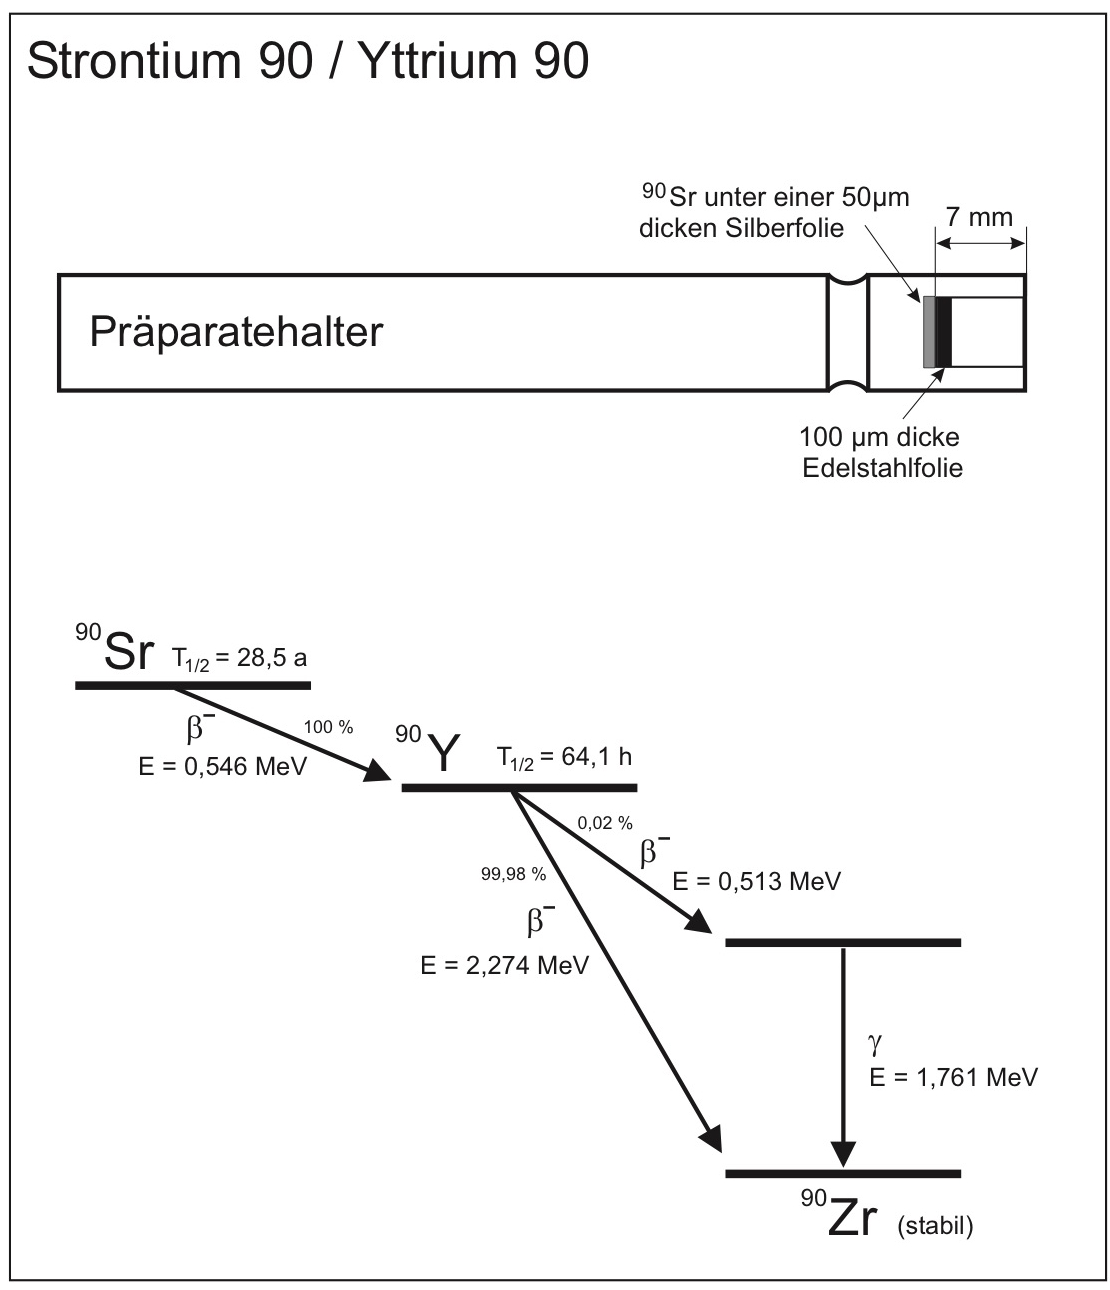
\includegraphics{graphics/PAP2_2-82.jpg}}
    \caption{Aufbau des Strontium Präparats und zugehöriges Zerfallsschema [Quelle: PAP2.2 Skript, S.82, Stand: 01.08.2024]}
    \label{fig:Anhang-Strontium}
\end{figure}

\begin{figure}[!p]
    \centering
    \resizebox{0.9\textwidth}{!}{
    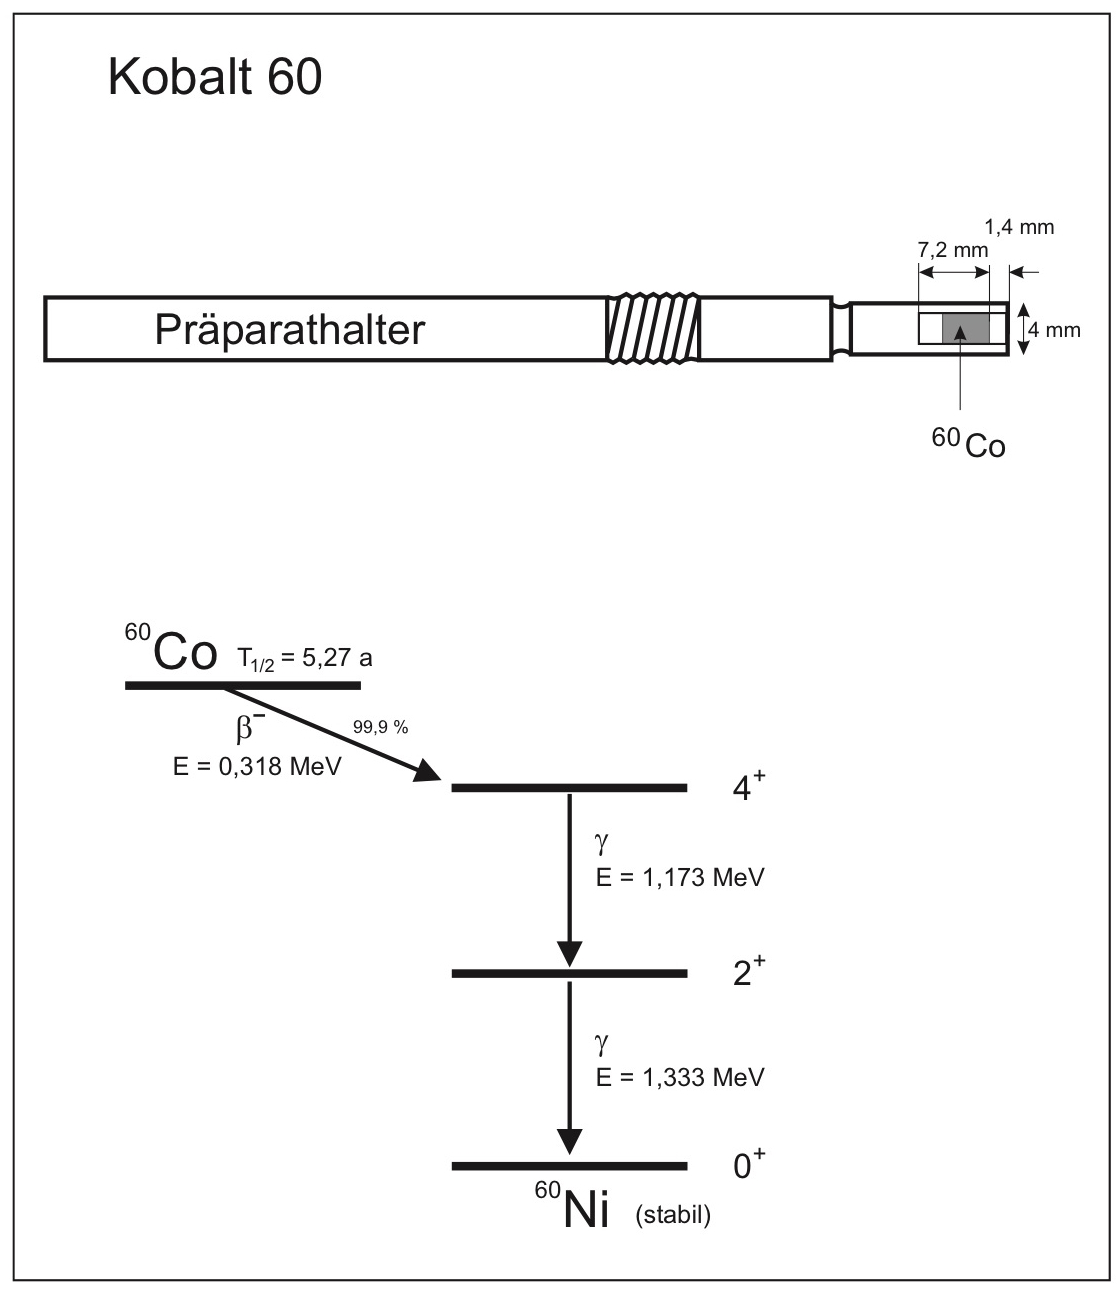
\includegraphics{graphics/PAP2_2-83.jpg}}
    \caption{Aufbau des Kobalt Präparats und zugehöriges Zerfallsschema [Quelle: PAP2.2 Skript, S.83, Stand: 01.08.2024]}
    \label{fig:Anhang-Kobalt}
\end{figure}


\begin{figure}[!p]
    \centering
    \resizebox{0.9\textwidth}{!}{
    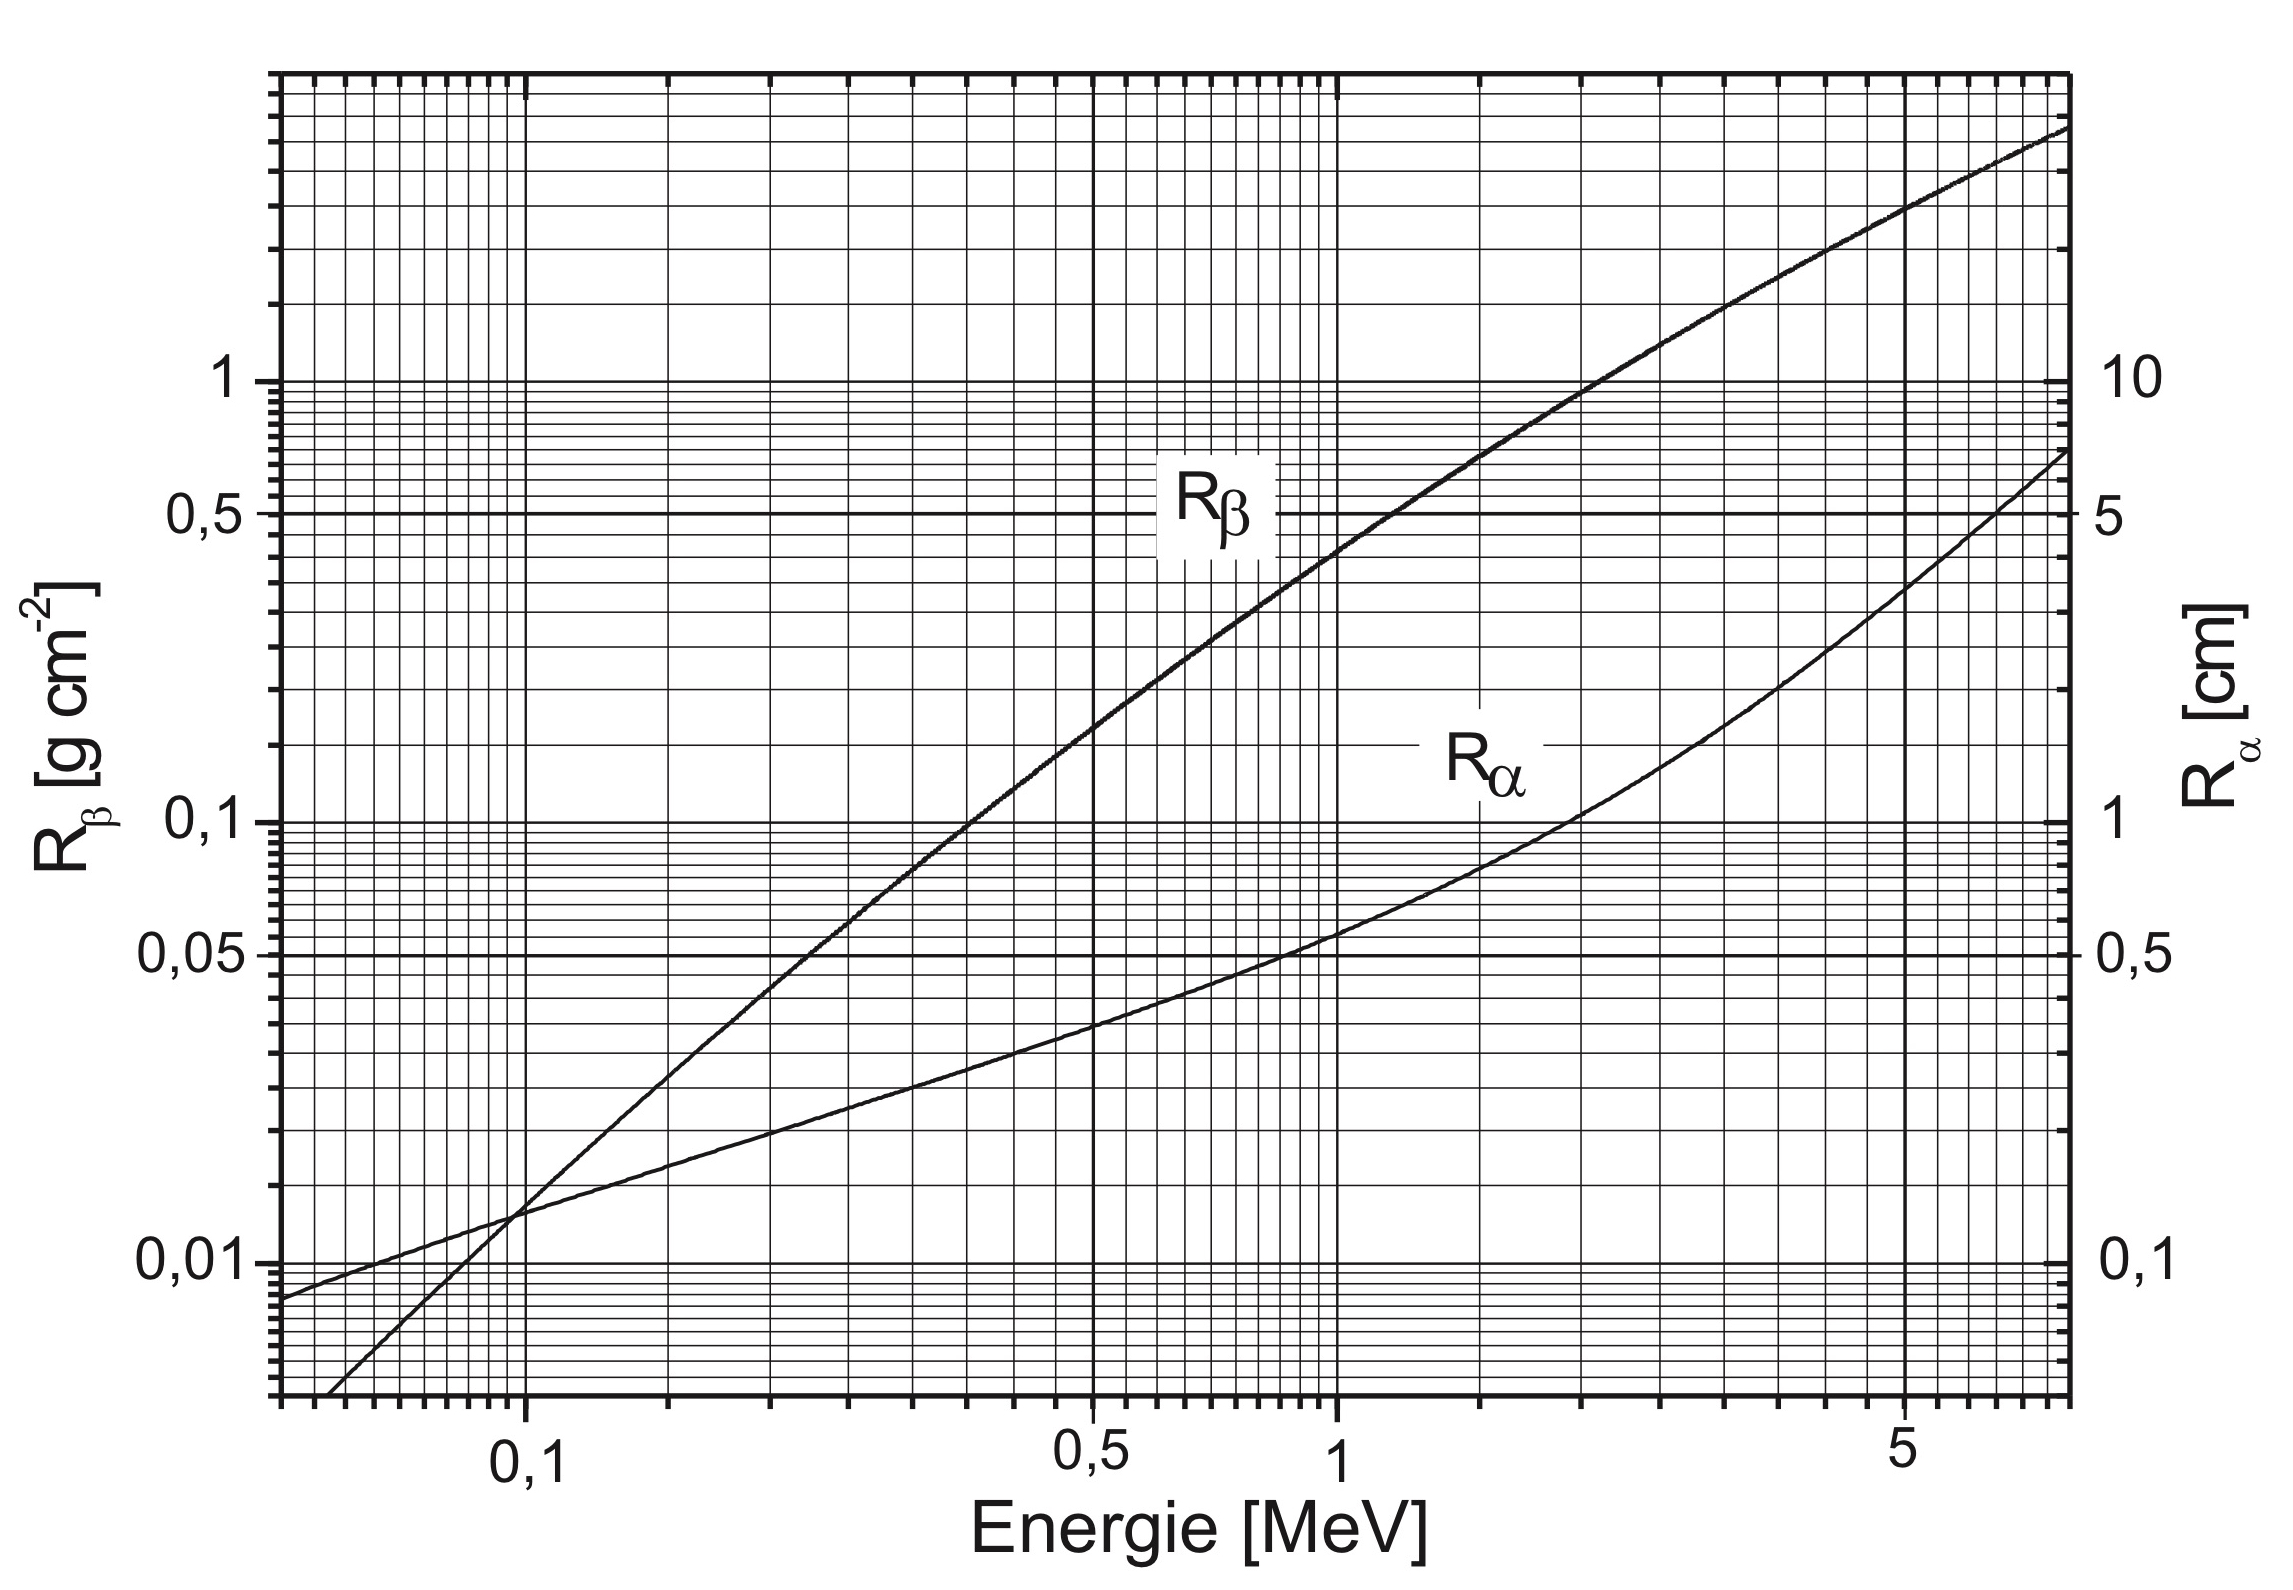
\includegraphics{graphics/PAP2_2-84.jpg}}
    \caption{Reichweite von $\beta$-Strahlung in Aluminium von und $\alpha$-Strahlung in Luft [Quelle: PAP2.2 Skript, S.84, Stand: 01.08.2024]}
    \label{fig:Anhang-Reichweite}
\end{figure}


\begin{figure}[!p]
    \centering
    \resizebox{0.9\textwidth}{!}{
    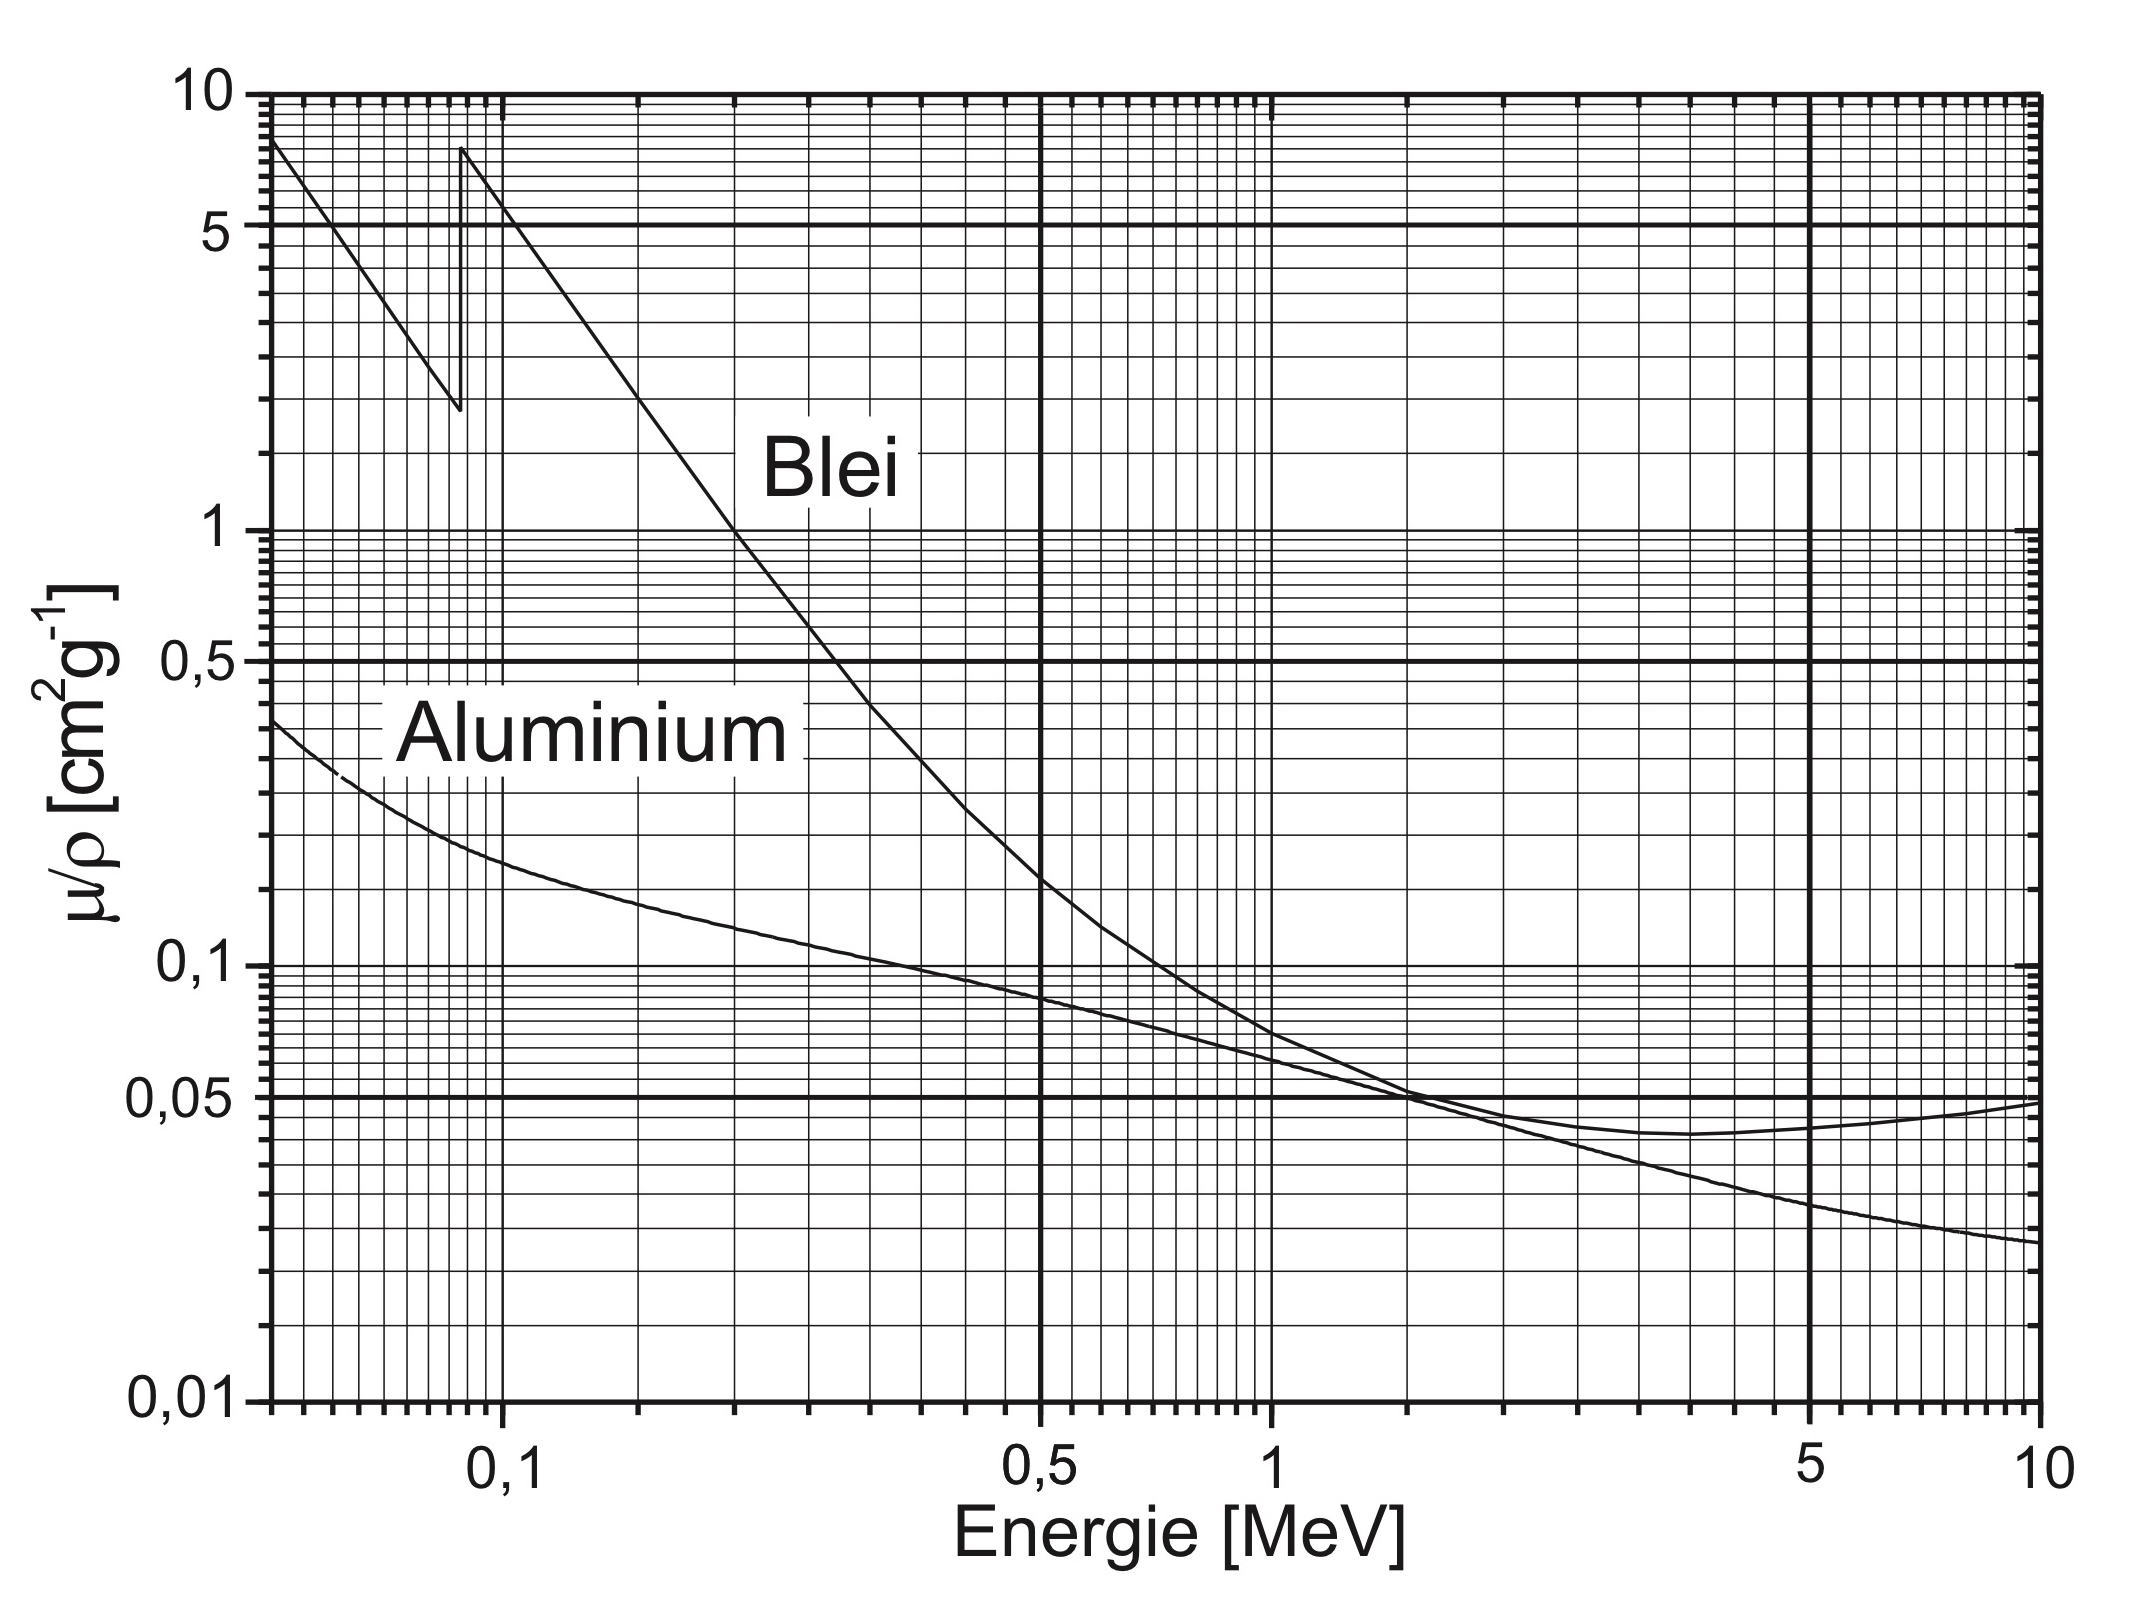
\includegraphics{graphics/PAP2_2-85.jpg}}
    \caption{Photon Cross Section from 1 keV to 100 MeV for elements Z=1 to 100 [Quelle: PAP2.2 Skript, S.85, Stand: 01.08.2024]}
    \label{fig:Anhang-PhotonCrossSection}
\end{figure}

\newpage
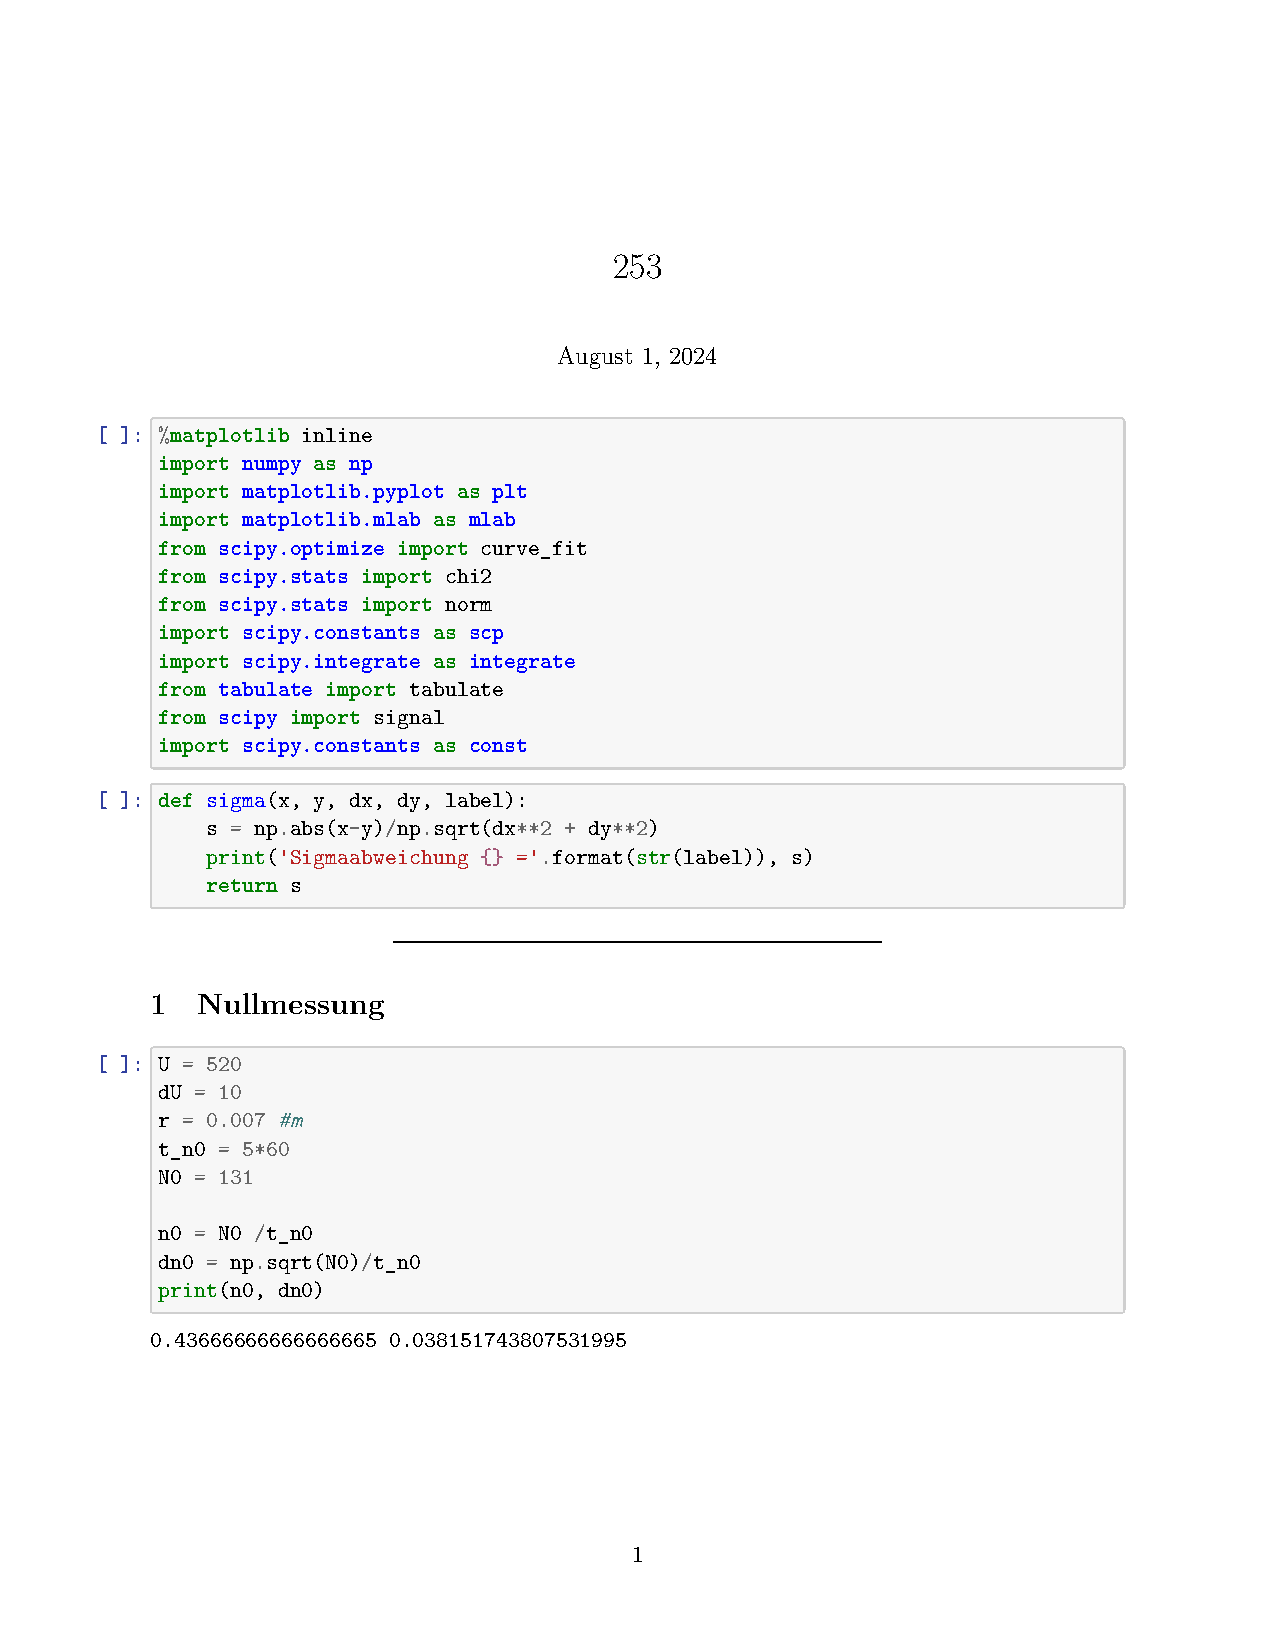
\includepdf[pagecommand=\invisiblesection{Python-Code},scale=0.8,pages=1]{253.pdf}
\includepdf[pagecommand={},scale=0.8,pages=2-last]{253.pdf}

\end{document}

